%% 
%% Copyright 2007-2019 Elsevier Ltd
%% 
%% This file is part of the 'Elsarticle Bundle'.
%% ---------------------------------------------
%% 
%% It may be distributed under the conditions of the LaTeX Project Public
%% License, either version 1.2 of this license or (at your option) any
%% later version.  The latest version of this license is in
%%    http://www.latex-project.org/lppl.txt
%% and version 1.2 or later is part of all distributions of LaTeX
%% version 1999/12/01 or later.
%% 
%% The list of all files belonging to the 'Elsarticle Bundle' is
%% given in the file `manifest.txt'.
%% 
%% Template article for Elsevier's document class `elsarticle'
%% with harvard style bibliographic references

\documentclass[preprint,12pt,authoryear]{elsarticle}

%% Use the option review to obtain double line spacing
%\documentclass[authoryear,preprint,review,12pt]{elsarticle}

%% Use the options 1p,twocolumn; 3p; 3p,twocolumn; 5p; or 5p,twocolumn
%% for a journal layout:
%% \documentclass[final,1p,times,authoryear]{elsarticle}
%% \documentclass[final,1p,times,twocolumn,authoryear]{elsarticle}
%% \documentclass[final,3p,times,authoryear]{elsarticle}
%% \documentclass[final,3p,times,twocolumn,authoryear]{elsarticle}
%% \documentclass[final,5p,times,authoryear]{elsarticle}
%% \documentclass[final,5p,times,twocolumn,authoryear]{elsarticle}

%% For including figures, graphicx.sty has been loaded in
%% elsarticle.cls. If you prefer to use the old commands
%% please give \usepackage{epsfig}

%% The amssymb package provides various useful mathematical symbols
\usepackage{amssymb}
%% The amsthm package provides extended theorem environments
%% \usepackage{amsthm}

\usepackage{siunitx}  % for degree celsius
\usepackage{multirow} % for the table
\usepackage{booktabs} % fot toprule, midrule
\usepackage{longtable}

\usepackage{color,soul} % highlight 

\usepackage{hyperref} %for breaking long url

%% The lineno packages adds line numbers. Start line numbering with
%% \begin{linenumbers}, end it with \end{linenumbers}. Or switch it on
%% for the whole article with \linenumbers.
%% \usepackage{lineno}

\usepackage{lineno}
\linenumbers

\journal{Remote Sensing of Environment}

\begin{document}

\begin{frontmatter}

%% Title, authors and addresses

%% use the tnoteref command within \title for footnotes;
%% use the tnotetext command for theassociated footnote;
%% use the fnref command within \author or \address for footnotes;
%% use the fntext command for theassociated footnote;
%% use the corref command within \author for corresponding author footnotes;
%% use the cortext command for theassociated footnote;
%% use the ead command for the email address,
%% and the form \ead[url] for the home page:
%% \title{Title\tnoteref{label1}}
%% \tnotetext[label1]{}
%% \author{Name\corref{cor1}\fnref{label2}}
%% \ead{email address}
%% \ead[url]{home page}
%% \fntext[label2]{}
%% \cortext[cor1]{}
%% \address{Address\fnref{label3}}
%% \fntext[label3]{}

%\ead{huanglingcao@link.cuhk.edu.hk}

\title{Mapping Retrogressive Thaw Slumps in the Beiluhe Region (Tibetan Plateau) from CubeSat images using Deep Learning}

%% use optional labels to link authors explicitly to addresses:
%% \author[label1,label2]{}
%% \address[label1]{}
%% \address[label2]{}

\author[a]{Lingcao Huang}
\author[b]{Jing Luo}
\author[b]{Zhanju Lin}
\author[b]{Niu Fujun}
\author[a]{Lin Liu}


\address[a]{Earth System Science Programme, Faculty of Science, The Chinese University of Hong Kong, Hong Kong SAR, China.}
\address[b]{Northwest Institute of Eco-Environment and Resources, Chinese Academy of Sciences, LanZhou, China.}

\begin{abstract}

Retrogressive thaw slumps (RTS) are one of the most dynamic landforms in the permafrost areas, and their formation attributes to the thawing of ice-rich permafrost. The spatial distribution and impacts of RTSs on the Tibetan Plateau are poorly understood because of their remote locations and technical challenges in automatic mapping. In this study, we innovatively applied the-state-of-art deep learning algorithms to Planet CubeSat images, which are satellite images with high the spatial and temporal resolution. Our objectives are to (1) automatically map RTSs in the Beiluhe region on the Tibetan Plateau from the CubeSat images and (2) analyze the relation between the spatial distribution of RTSs and terrain factors. Our method allows us to delineate 196 RTSs automatically with the average precision of 0.536 and the corresponding precision, recall, and F1 score are 0.842, 0.817, and 0.829, respectively (under the IOU threshold of 0.5). The analysis of the spatial distribution shows that (1) most of the RTSs are small ( area < eight ha) and the perimeters are smaller than 2000 meters and (2) RTSs preferentially develop at locations with relative high elevation, gentle slopes, relatively lower than the surroundings, and receiving less solar radiations. The results show that the method can map RTS automatically from Planet CubeSat images and has the potential of applying to larger areas.  

%1) the method (2)

\end{abstract}

\begin{keyword}
%% keywords here, in the form: keyword \sep keyword

%% PACS codes here, in the form: \PACS code \sep code

%% MSC codes here, in the form: \MSC code \sep code
%% or \MSC[2008] code \sep code (2000 is the default)
Convolutional neural network \sep Planet CubeSat  \sep Permafrost thawing  \sep Retrogressive Thaw Slumps \sep Tibetan Plateau.

\end{keyword}

\end{frontmatter}

%% \linenumbers
%\tableofcontents

%% main text
\section{Introduction}
\label{sec_intro}

Permafrost underlies approximately 24\% of the exposed land surface in the northern hemisphere \citep{zhang_statistics_1999} and undergoes warming as well as degradation. Records in the borehole measurement show that the permafrost is undergoing strong warming \citep{marchenko_permafrost_2007,osterkamp2005recent,romanovsky_thermal_2010,romanovsky_permafrost_2010,wu_recent_2008,zhao_thermal_2010}. Warming of permafrost can cause its degradation such as active layer thickening, shrinking in its area, and development of thermokarst landforms \citep{zhao_thermal_2010,akerman_thawing_2008,czudek_thermokarst_1970,jorgenson_response_2005,osterkamp_characteristics_2007}. Permafrost degradation causes damage to infrastructure, increases net source of atmospheric carbon and significantly alters local ecosystem \citep{tong_effect_1996,grosse_vulnerability_2011,olefeldt_circumpolar_2016,schuur_climate_2015,tarnocai_soil_2009,schuster2018permafrost}. On the Tibetan Plateau, permafrost underlies over a total area of about 1.06$\times10^6$ $km^2$ and is shallow (thinner than 100 m) as well as warm (higher than \SI{-2}{\celsius}) \citep{zhou_geocryology_2000}. Therefore, permafrost on the Tibetan Plateau is sensitive and vulnerable to climate changes and anthropogenic disturbance. Mapping and monitoring the changes in permafrost areas are essential to understand the impacts and consequences of permafrost degradation. 

A retrogressive thaw slump (RTS) is one of over 20 types of thermokarst landforms resulting from the thawing of ice-rich permafrost \citep{czudek_thermokarst_1970, jorgenson_response_2005, jorgenson_thermokarst_2013,kokelj2013advances}. Several trigger mechanisms including lateral stream erosion and active layer detachments are responsible for RTSs \citep{french2017periglacial}. Commonly, a detachment slide removes the soil above permafrost and exposes it to rapid thawing, then initiates an RTS. Retrogressive thawing of permafrost at the exposed headwall further expands the thawed area toward upslope \citep{jorgenson_thermokarst_2013}. Typically, the maximum retreat rates are 6--8 meters per year \citep{jorgenson_thermokarst_2013}. Once an RTS initializes, it can be active for decades \citep{burn1989geomorphology, lacelle2010climatic, swanson2018growth} and has significant impacts on local and downslope ecosystem \citep{gooseff2009effects, pierre2018unprecedented, zolkos2018mineral}. %However, there are many RTSs in the unmapped permafrost areas and require intensive investigation. 

RTSs can occur throughout permafrost areas, but many of them are unmapped, especially those on the Tibetan Plateau. Many studies investigated RTSs in the northern and central Alaska \citep{swanson2018growth,gooseff2009effects,balser2014timing}, northern Canada \citep{burn1989geomorphology, lacelle2010climatic, ramage_terrain_2017, lantuit_fifty_2008, lacelle_distribution_2015, segal2016acceleration, brooker2014investigating, kokelj2017climate, obu2017coastal, ramage_increasing_2018, lantz2008increasing, brooker2014mapping, frappier2017retrogressive, zwieback2018sub, rudy2017terrain, armstrong2018thaw, kokelj2013thawing, rudy2016transferability, burn1990canadian,  cassidy2017impacts}, Siberia \citep{czudek_thermokarst_1970, zwieback2018sub, leibman2003dynamics} and the Tibetan Plateau \citep{wang1995situ, niu2005engineering, niu2012development, niu2014thaw, niu2016thaw, sun2017creep, ma2006slope}. Due to the limitations of mapping methods, these are site-focused or regional studies. Comparing to the Arctic and subarctic, there are much less investigations of RTSs on the Tibetan Plateau. A few studies focused on one or several RTSs near to the Qinghai-Tibet Highway. The only regional studies targeted an area along the Qinghai-Tibet Engineering Corridor \citep{niu2014thaw, niu2016thaw}. The distribution and impacts of RTSs in large permafrost areas on the Tibetan Plateau are poorly quantified and understood. The possible reasons are (1) most of them are in remote and inaccessible regions and (2) they are similar to the surroundings or other landforms, which make it challenging to map them on remote sensing images.  %TODO: more on RTS? what is the difference between RTS in QTP and Arctic?

The images from CubeSats enable us to map the spatial distribution of RTSs on the Tibetan Plateau. CubeSats, small and low-cost satellites, can provide high spatial and temporal resolution images by deploying them in a multi-satellite constellation. Planet (as known as Planet Labs; \url{planet.com}) has deployed more than 150 CubeSats in sun-synchronous orbit and collects images nearly all of the global land surface at 3--5 m resolution daily. These images have great potential for earth observation and have been used in many studies, such as water body tracking \citep{cooley2017tracking, cooley2019arctic, aragon2018cubesats, miles2018glacial}, vegetation \citep{houborg2016high, houborg2018daily}, and glacier investigation \citep{altena2017glacier}. In this study, we collect images of our study area from the PlanetScope constellation (hereafter referred to as “Planet images”), which have a spatial resolution of 3 m and are sufficient for visualizing most of the retrogressive thaw slumps. The high temporal resolution of Planet images ensure that we can acquire cloudless images covering the whole study area within one-month even there is frequent cloud cover. With the high spatial resolution, we can map many RTSs whose area around one ha or smaller such as the ones reported in \citep{niu2012development,niu2016thaw} and accurately delineate their boundaries. These small RTSs may be missed on Landsat images because of the coarse resolution (30 m) although they were used to mapped RTSs in circumpolar areas\citep{lacelle_distribution_2015, brooker2014mapping, nitze2018remote}. The accurate boundaries of RTSs are essential for quantifying their temporal changes. 

To automatically map RTSs, which is necessary for a large area, we innovatively apply deep learning algorithms to Planet images. Previous studies (e.g., \citealp{ramage_terrain_2017, lantuit_fifty_2008, niu2014thaw}) combined field investigation and manual delineation on high-resolution remote sensing images to obtain the inventories of RTSs, which are time-consuming and limited to small areas. Comparing to thermokarst lakes, RTSs are complex landforms and are challenging to be mapped automatically on images. An RTS consists of the headwall, slump floor, slump lobe, and headscarp \citep{lantuit_fifty_2008}. Different parts of RTSs have different colors on images because of various soil types, water content, incoming solar angles, and vegetation. In some regions with sparse vegetation, the colors of RTSs are quite similar to other land covers such as bare lands. Therefore, the diverse radiometric characteristics and the similarity to the surroundings of RTSs require a mapping method which has the high capability and can represent their unobvious features. Deep learning is such a kind of methods and has achieved unprecedented results in many fields such as computer vision and artificial intelligence \citep{krizhevsky_imagenet_2012, lecun_deep_2015, silver_mastering_2017}. In remote sensing applications, deep learning also achieved exceptionally good results in land cover mapping, object detection, poverty estimation, and delineation of ice-wedge polygons \citep{jean_combining_2016, guo_geospatial_2018, zhang2018deep}. However, none of these studies have targeted RTSs. 

The objectives of this study are: (1) to automatically map RTSs on Planet images based on deep convolutional neural networks and (2) to analyze the relation between the spatial distribution and terrain factors in the Beiluhe region on the Tibetan Plateau. We innovatively applied DeepLab V3+, a state-of-the-art semantic segmentation algorithm, to Planet images and conducted numerous experiments using different hyper-parameters. By comparing to manual delineations, we calculated the accuracies of mapping results and assess the performance of our method. Based on the mapping results, we quantified their geometric characteristics and analyzed the relation between their spatial distribution and terrain factors. Lastly, we will discuss the advantages and limitations of using Planet images as well as the automatic mapping method.  


\section{Study area}
\label{sec_studyarea}
The study area ($92.50^\circ$E to $93.51^\circ$E, $34.69^\circ$N to $35.18^\circ$N) is in the Beiluhe region on the Tibetan Plateau (Fig. \ref{fig_rts_groundphoto}) with an approximate size of 7500 $km^2$. The elevation ranges from 4418 m to 5320 m with a mean of 4673 m. The record from a nearest (5km to the northern edge) meteorological station shows that the mean annual air temperature and annual precipitation are \SI{-3.8}{\celsius}, and around 300 mm, respectively \citep{luo_thermokarst_2015}. The vegetation includes alpine meadow (\textgreater 45\%) and alpine grassland (\textless 20\%) \citep{luo_thermokarst_2015}. 

Most of this area is underlain by ice-rich permafrost: 70\% of the area with ice contents \textgreater 30 \%, while 20\% has ice contents \textgreater 50\%, and the thickness of permafrost ranges from 20 to 80 m \citep{zhou_geocryology_2000, luo_thermokarst_2015}. The mean annual ground temperature of the entire area is between \SI{-2.0} and \SI{-0.5}{\celsius}, and the active layer thickness is between 1.5 and 2.0 m \citep{zhou_geocryology_2000, luo_thermokarst_2015, wu2010changes, wu2015changes}. \hl{ More information? (air/ground temperature change?)}  %TODO: more information on study area

\begin{figure}[ht]
	\centering
	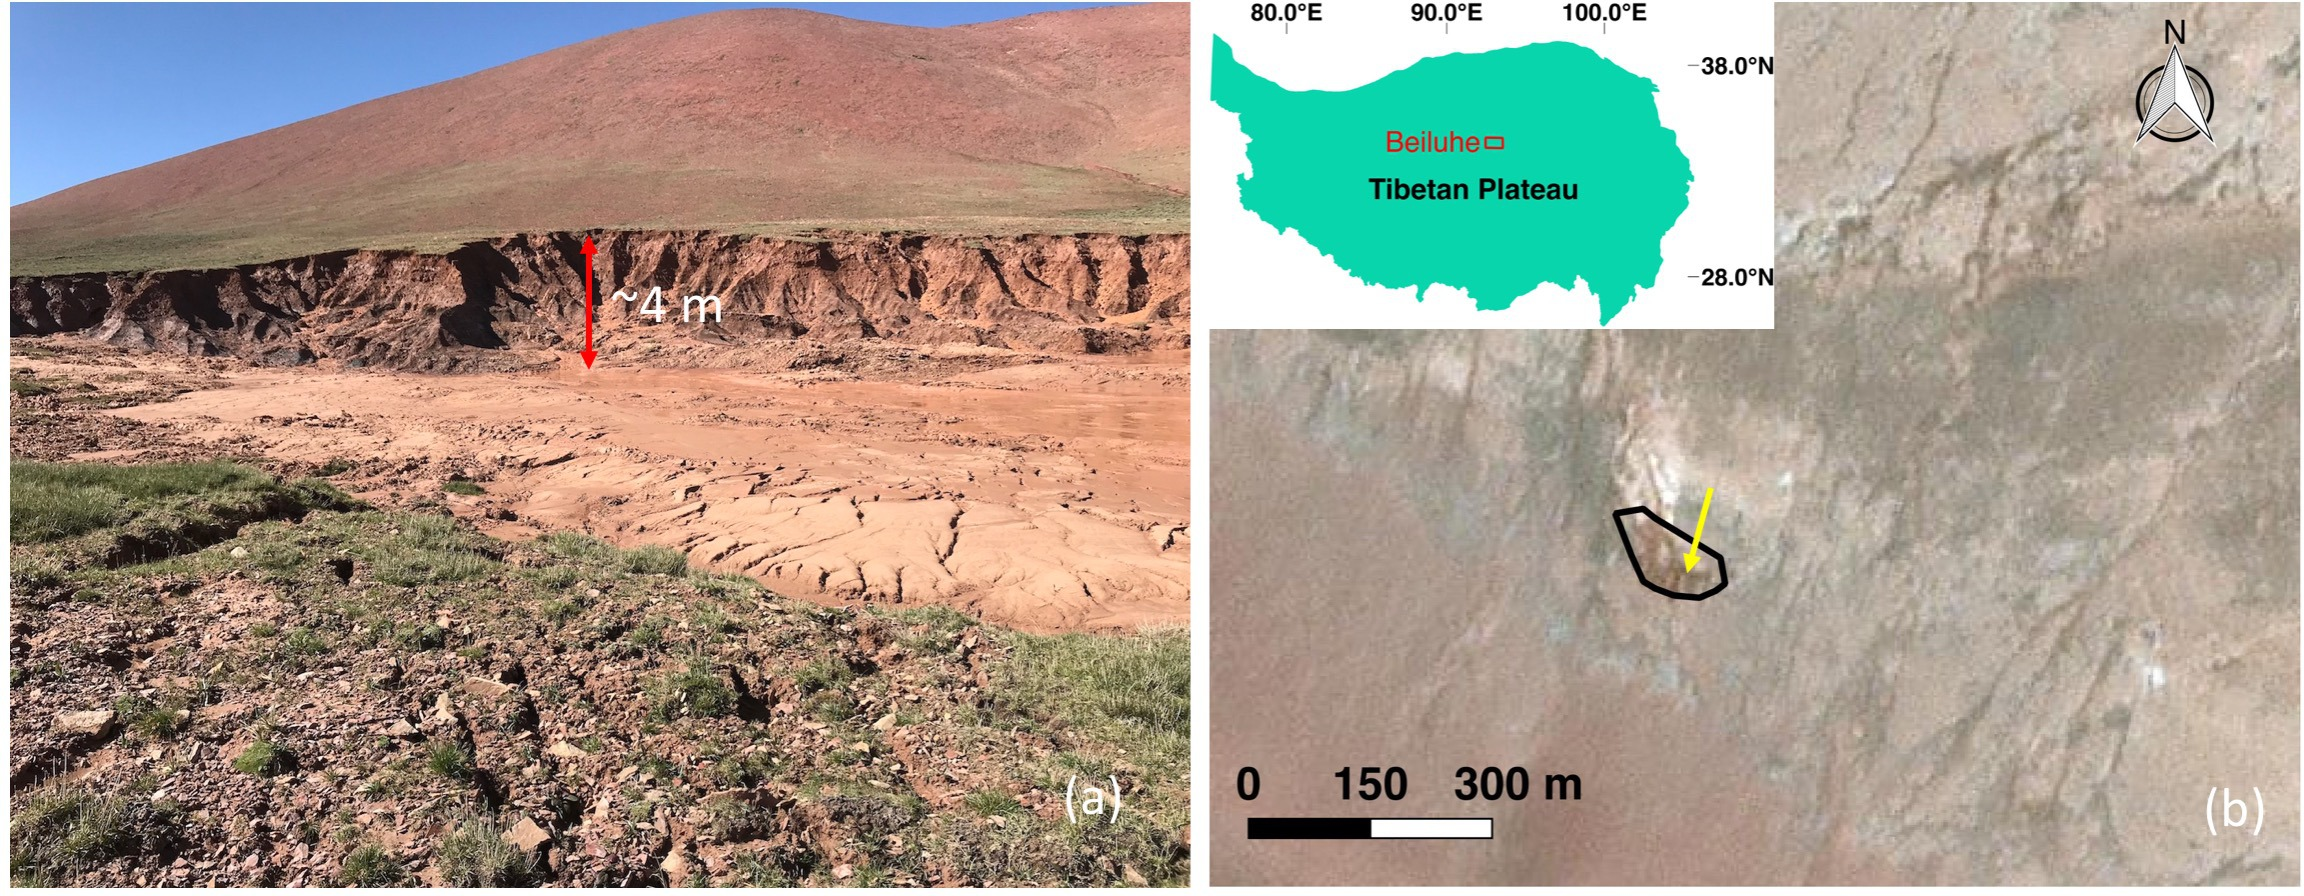
\includegraphics[width=14cm]{figures/study_area_loc_RTS_photo_trim.jpg}
	\caption{The ground photo (a) and Planet image (b) of a retrogressive thaw slump (RTS). In (b), the black polygon outlines the RTS, the yellow arrow indicates the looking direction of the ground photo, and the inset shows the location of our study area.}
	\label{fig_rts_groundphoto}
\end{figure}

RTSs are one of the typical thermokarst landforms in this area. Fig. \ref{fig_rts_groundphoto}a shows the ground photo of an RTS. The headwall height and the size of the RTS is around four meters and 0.9 ha, respectively. Fig. \ref{fig_rts_groundphoto}b shows the corresponding remote  image, which is a subset of Planet images with red, green, and blue bands. 

\section{Methods}
\label{sec_meth}

\subsection{Collection and Pre-processing of Planet images}
\label{subsec_collect_images}

We downloaded Planet images via the Planet website (\url{www.planet.com}). The Planet’s Education and Research Program allows us to download images covering up to 10,000 $km^2$ without charge. We downloaded 64 PlanetScope scenes of images (as known as Daily Imagery), and each scene covers an area of around 10 km by 30 km and has four bands (blue, green, red, and near-infrared).  The acquisition dates were 22 and 23 May 2018. The product level we chose was “Analytic”, which means that the images have been orthorectified and converted to Surface Reflectance. Moreover, the bit depth and positional accuracy are 16 bit and higher than 10 m, respectively. Planet also provides mosaic images but only available for commercial request. 

We pre-processed the Planet images according to the requirement of the deep learning algorithm and manual delineation. For the 64 scenes, we mosaicked and extracted red, blue, and green (RGB) bands using Geospatial Data Abstraction Library (GDAL, \url{gdal.org}), then stretched and sharpened the images using OpenCV (\url{opencv.org}). Since the deep learning algorithm used in this study only accept three bands of images, we conducted experiments to decide the best approach to extract three bands from Planet images. The potential approaches include (1) extracting RGB bands since they are the natural color and will make manual identification easy, (2) combining of normalized difference vegetation index (NDVI) \citep{rouse1974monitoring}, normalized difference water index (NDWI) \citep{mcfeeters1996use}, and the blue band (excluded when calculating NDVI and NDWI), and (3) adopting the first three components after principal component analysis (PCA). Formation of RTSs results in the abrupt change of land cover in vegetation and soil moisture, therefore, the combination of NDVI and NDWI can help identify RTSs on images. PCA is a statistical procedure that re-organizes the information in a descending order \citep{wold1987principal}. By using PCA, we can keep the most information of Planet images when converting the original images to three bands. We adopted the approach of extracting RGB bands for pre-processing because it achieved the highest accuracy (see section \ref{subsub_otherbands}). After pre-processing, we obtained a single image whose size is 30916 pixels by 18713 pixels as the input for the automatic mapping method and manual delineation. 

\subsection{Collection of Ground Truth Polygons}
\label{subsec_collect_groundtruth}

We manually delineated RTSs on Planet images in QGIS (version 2.18.14, \url{qgis.org}) and conducted fieldwork to validate them. We divided the entire study area to 1410 vector grids, and the size of each grid is 2.3 km$\times$2 .3km. RTSs in each grid were independently delineated by two researchers who have extensive experiences in mapping RTSs. Any inconsistent result in each grid would be discussed and decided with the third researcher. The criteria for mapping RTSs are based on their distinct morphologic and tonal characteristics including the presence of a headwall, slump floor, or toe, the absence of vegetation, and the shape. We cross-checked 90\% of the manual results in field work of 2014 as well as 2018 and all of them in Google Earth. Lastly, we obtained 202 polygons of RTSs as ground truths.  

\subsection{Automatic mapping of RTSs}
\label{subsec_auto_mapping}

Fig. \ref{fig_flowchart} shows the flowchart of our automatic mapping method. Firstly, we converted boundaries of landforms (i.e., ground truths) and a portion of Planet images to training images and label images. Secondly, we trained the neural network and obtained its parameters which have learned features from the training data. Lastly, we inputted the Planet image of our study area and predicted RTSs. After post-processing, we obtained mapped polygons of RTSs. Lastly, we validated the mapped polygons and calculated the accuracy. The details of each step will be described as follows. %TODO: add word which would be used in the whole text. 

\begin{figure}[ht]
	\centering
	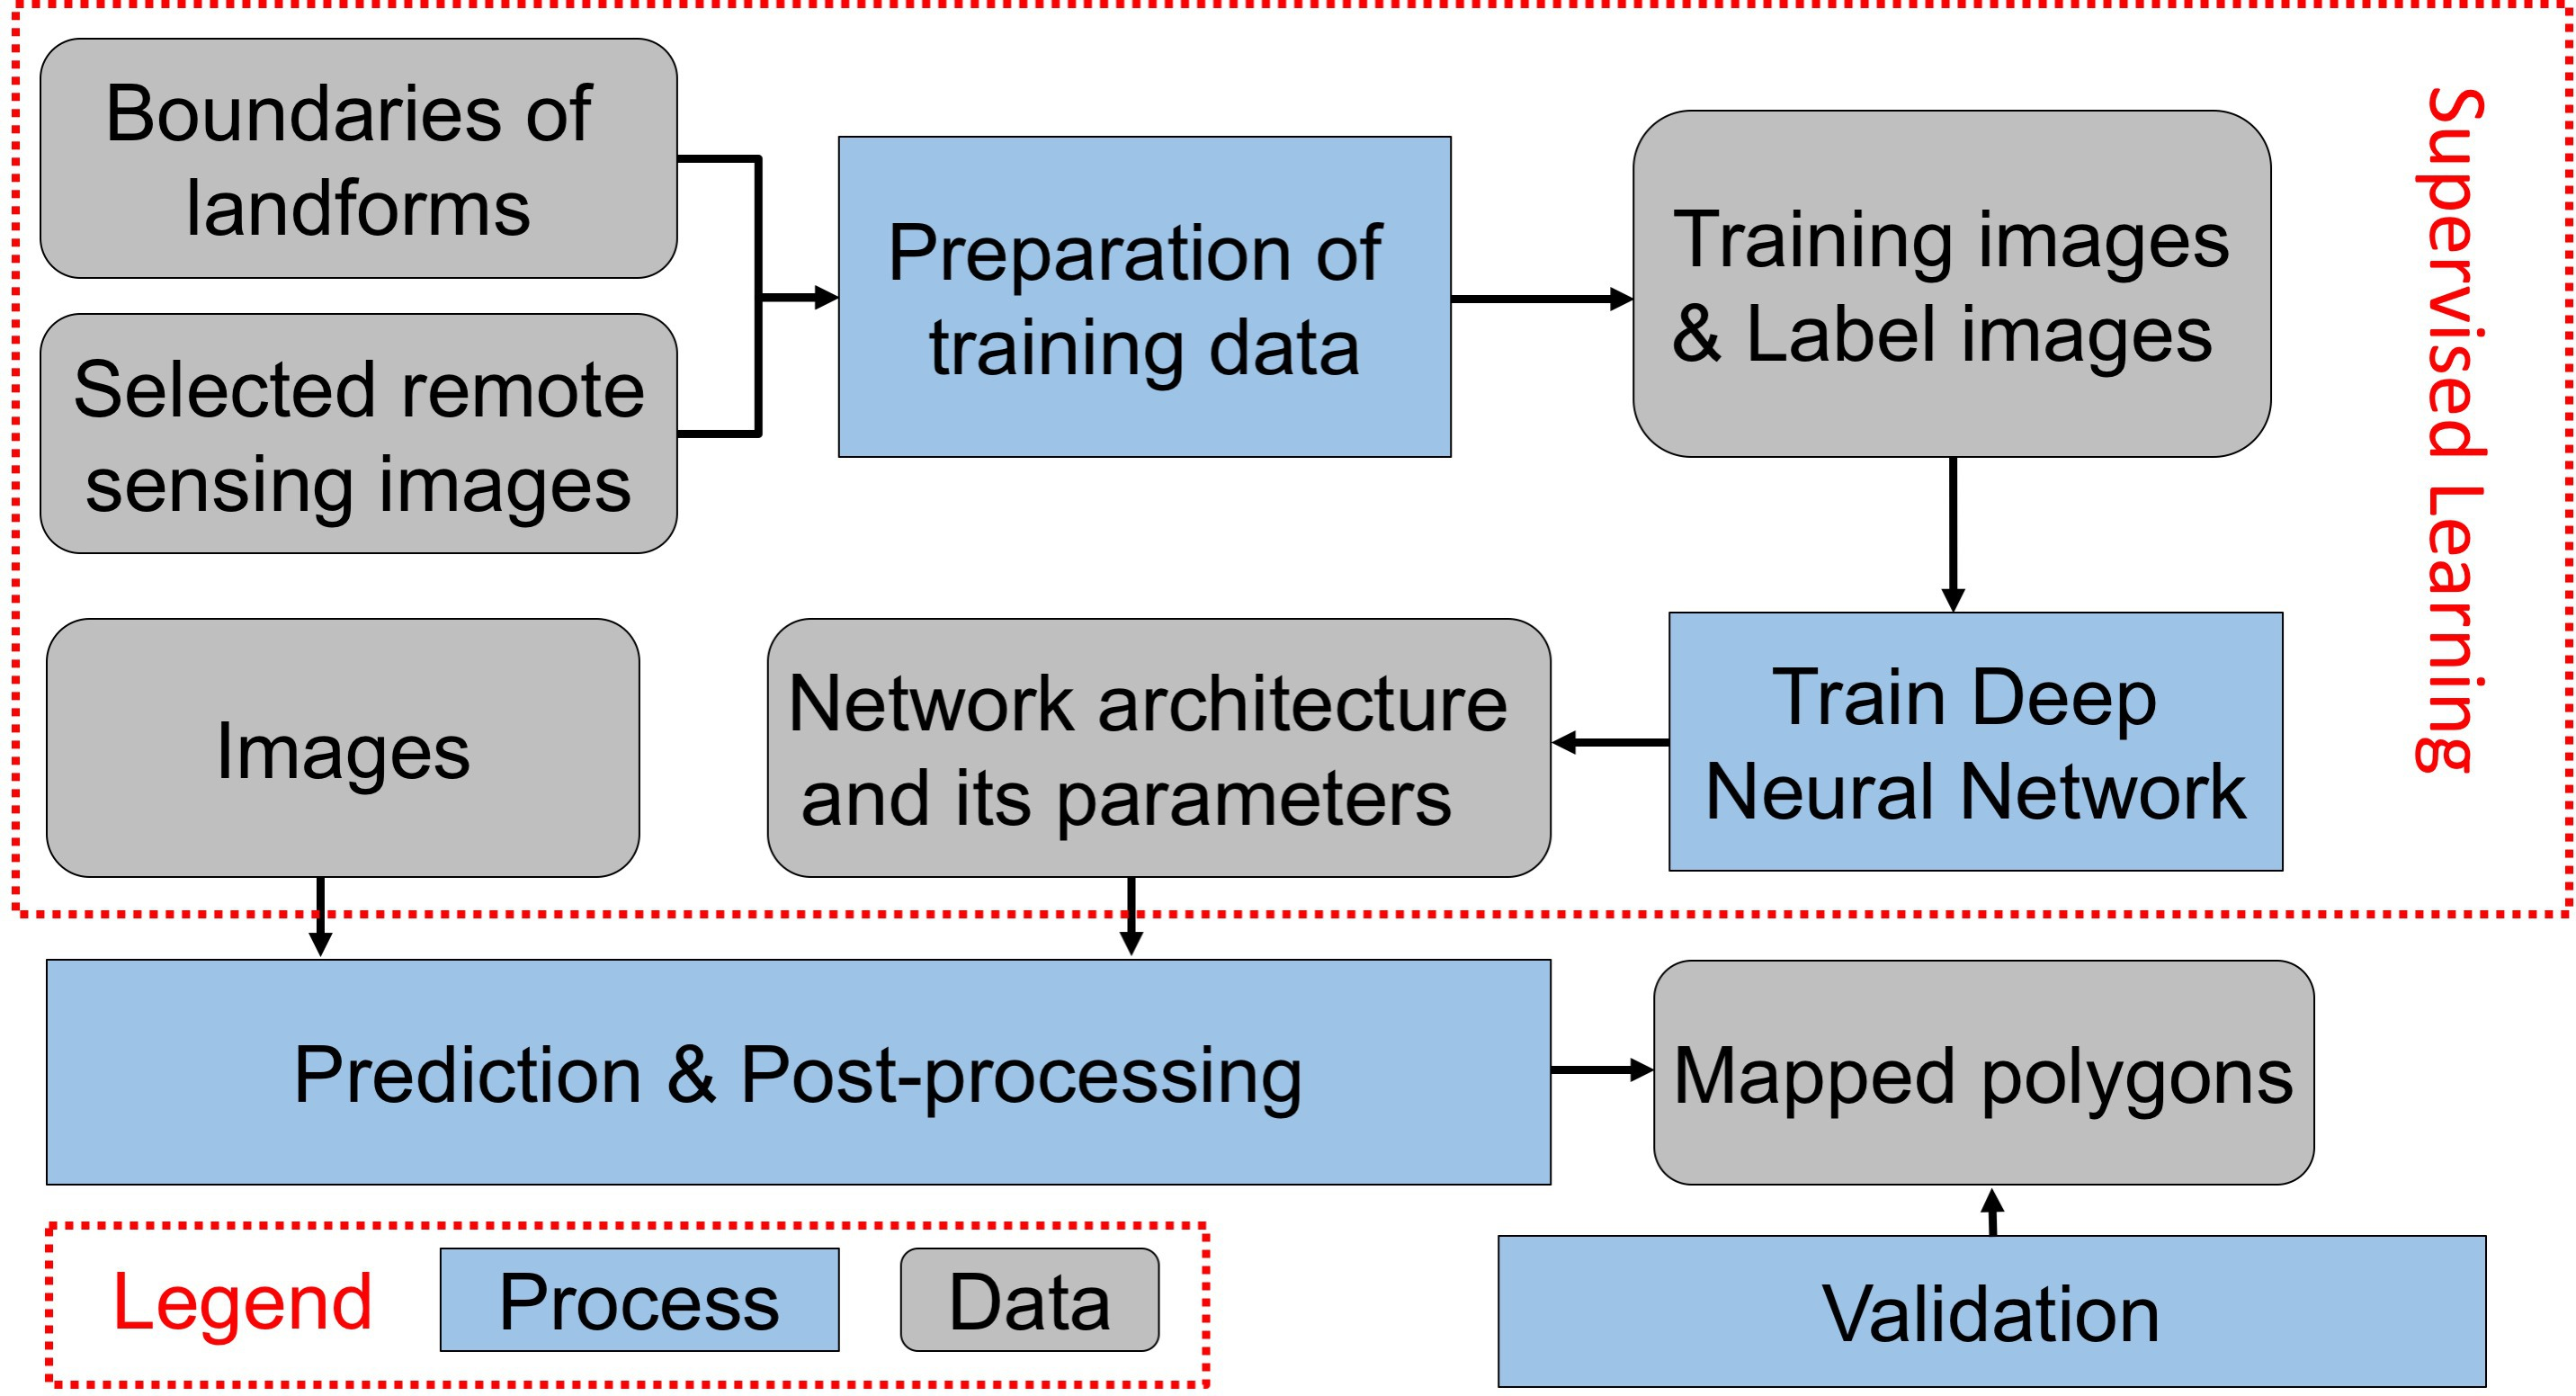
\includegraphics[width=12cm]{figures/flowchart_trim.jpg}
	\caption{Flowchart of the automatic mapping method based on deep learning algorithms.}
	\label{fig_flowchart}
\end{figure}

\subsubsection{Preparation of training data}
\label{subsubsec_pre_trainingdata}

We derived training data by choosing all the ground truths as positive training polygons and 104 non-RTS polygons as negative ones. The non-RTS polygons cover areas where do not have any RTS but other land covers such as vegetation, bare land, and water bodies. To make the non-RTS polygons representative for training, we ran an initial mapping process excluding negative samples, then we drew non-RTS polygons cover areas where contains many incorrect results. This is practical to choose negative samples that are similar to RTSs. Since the surrounding area of an RTS is critical for our method, we set a buffer area of 300 meters and then extracted sub-images of positive and negative training polygons. Figure S1, S2, and S3 in the Supplementary Materials show the distribution and extents of training polygons and sub-images. The sub-images only cover 6.03\% (1.35\% and 4.68\% derived from positive and negative training polygons, respectively) of the entire study area. Furthermore, we subdivided a sub-image to patches by setting a patch size as 480 pixels with an overlap of 160 pixels. More details of deriving training images and label images from the training polygons can be found in \cite{huang2018automatic}. 

%TODO: move to discussion: Similarly, we can collect training data in several case studies, and then map RTSs on the entire Tibetan Plateau.

To improve the number of training data and generalization of the method, we applied data augmentation to the positive patches. We excluded the negative patches during data augmentation because their quantities are sufficient for training. The most common data augmentation practices include flipping, blurring, cropping, scaling, and rotating. In this study, we utilized the implementation of these strategies in the “imgaug” package (\url{imgaug.readthedocs.io}). Specifically, we adopted flipping (left and right as well as up and down), blurring (gaussian blur with sigma equal to one and two), cropping (10 and 30 pixels), scaling (with factors are 0.75 and 1.25), and rotating (45, 90, and 135 degrees). Since effectiveness and methods of data augmentation depend on the application domain \citep{perez2017effectiveness}, we conducted a set of experiments of applying different combinations of data augmentation methods (results in section \ref{subsub_accuracies}). Based on the experiments, we only adopted flipping, blurring, cropping of the data augmentation. 

\subsubsection{Training, prediction, and post-processing}
\label{subsubsec_deeplab}

The automatic mapping method is a supervised learning method and built on DeepLabv3+ \citep{chen_encoder-decoder_2018}, which is a state-of-the-art deep learning algorithm for semantic segmentation. Semantic segmentation implies the algorithm will give each pixel a class label to indicate the its category on images. Similarly, our goal is to label each pixel on the Planet image as RTS or non-RTS. DeepLabv3+ is the latest version of DeepLab and outperforms many other algorithms in the VOC image segmentation tasks \citep{everingham_pascal_2015}. Moreover, the implement of DeepLabv3+ is open source and available on Github (\url{github.com/tensorflow/models/tree/master/research/deeplab}).

Training is an iterative process and make the network of DeepLabv3+ learn features from training data. The network architecture we used is Xception65 \citep{chollet2017xception}, and the pre-trained model is based on the ImageNet datasets \citep{russakovsky2015imagenet}. The learning rate is 0.007, and iteration number is 30000. To evaluate the robustness of this algorithm, we utilized 5-fold and 10-fold cross-validation, which are commonly used in machine learning. In the 5-fold cross-validation, we randomly divided the positive and negative training polygons to five portions with a roughly equal count and then used four portions for training and the remaining one for validation. We repeated this training processing five times and presents the results in Figure S4 of the Supplementary Materials. Figure S5 in the Supplementary Materials shows that average precision in 10-fold cross-validation is slightly higher than the one in 5-fold, which indicates that more training data (90\% in 10-fold and 80\% in 5-fold) can lead to better results. To achieve the best results, we included all the ground truths as training polygons and applied data augmentation to training data. 
%TODO: marker, stop here. 
We divided the Plant images into many small patches (480 pixels $\times$  480 pixels) and inference on each patch, then merged the result of each patch and converted to mapped polygons using GDAL. More details on how to convert inference patches to mapped polygons can be found in \cite{huang2018automatic}. Lastly, we removed mapped polygons whose area is smaller than 0.3 ha with the consideration of the image resolution.  

\subsubsection{Validation of automatic mapping results}
\label{subsubsec_validation}

We conducted two types of validation: pixel-based and polygon-based. The pixel-based method validates the results pixel by pixel and obtains the confusion matrix, kappa index, and overall accuracy index. The polygon-based method compares the mapped polygons to the ground truth polygons by using the intersection over union (IOU) method. The pixel-based accuracies are straightforward for comparison to other methods because it is widely used in the classification of remote sensing images. The polygon-based validation is more practical since the direct input and output of the method are the boundaries of RTSs. We used “Orfeo Tool Box” \citep{inglada2009orfeo} to conduct pixel-based validation with raster files of ground truths and mapped polygons. IOU is defined as 
\begin{equation}
IOU(A,B)=area(A \cap B)/area(A \cup B)
\label{equ_iou}
\end{equation}
where \emph{A} is a mapped polygon and \emph{B} is a ground truth polygon. A mapped polygon is a true positive if its value of IOU is greater than 0.5. Otherwise, it is a false positive. A missed ground truth is a false negative, i.e., the IOU value of the ground truth is zero. Furthermore, we can calculate
\begin{equation}
Precision=TP/(TP+FP)
\label{equ_precision}
\end{equation}
\begin{equation}
Recall=TP/(TP+FN)
\label{equ_recall}
\end{equation}
\begin{equation}
F1=2 \times Precision \times Recall / (Precision + Recall)
\label{equ_f1score}
\end{equation}
where \emph{TP}, \emph{FP}, and \emph{FN} are the numbers of true positives, false negatives, and false negatives. 

To evaluate the performance of the proposed method, we plot the precision-recall curve, which shows the relation between precision and recall for different thresholds. The precision-recall is a useful metrics to measure the success of prediction when the classes are imbalanced. In this study, RTSs occupy a very small portion of the entire area and are considered as one class, while other regions are non-RTS, i.e., the other classes. A high precision but low recall implies that the results contain few mapped polygons, but most of them are correct when compared to the ground truths. Conversely, a high recall but low precision implies that the results contain many mapped polygons, but most of them are incorrect. A set of good results requires high scores for both, that is, contain many results, and most of them are correct. The area under the precision-recall curve can be represented as average precision (AP):
\begin{equation}
AP=\sum_{i=2}^{n} (Recall_i - Recall_{i-1})\times Precision_i 
\label{equ_ap}
\end{equation}
to evaluate the method, where \emph{n} is the total number of thresholds for plotting the curve. 


\subsection{Quantification of RTS characteristics and terrain factors}
\label{subsec_quantify_rts}

We quantified the geometric characteristics of RTSs in the study area. Based on the mapped polygons of RTSs, we calculate their surface areas (\emph{S}), perimeters (\emph{P}) and circularities (namely, $\frac{4 \pi S}{P^2} $). The circularity is a metric to represent the shape of a polygon. Its value ranges from zero to one, and a polygon close to a perfect circle has the high circularity. In contrast, the value of a narrow polygon or starfish footprint is much less than one. 

To understand the relation between the spatial distribution and terrain factors, we quantified the terrain variables of RTSs, including elevation, slope, slope orientation, topographic position index (TPI), potential incoming solar radiation (PISR). The digital elevation model (DEM) we used is the 30 m SRTM \citep{farr2007shuttle}. The acquisition date of SRTM is in 2000, while most of the RTS in the study area were triggered after 2010 by checking the historical imagery in Google Earth. Therefore, the formation of RTSs would not affect the DEM. We used System for Automated Geoscientific Analyses, shorted as SAGA \citep{conrad2015system} to calculate these terrain variables. Slope, TPI, and PISR are in raster format with the same resolution as SRTM. The value is the mean value of pixels in the extent of an RTS. We defined a line segment of each RTS with its start point in the upslope and then calculated its azimuth as the slope orientation for the corresponding RTS. TPI is the difference between the elevation of a pixel and the surrounding defined by a specified radius \citep{guisan1999glm, reu2013application}. We set the radius as 100 meters in SAGA. A positive TPI indicates the pixel is higher than its surrounding, while a negative one for a lower location. PISR represents the received solar radiation, which can be affected by the topography and location. The difference in PISR can result in the variations in temperature, evaporation, patterns of snowmelt \citep{bohner2009land}. We calculated daily average of PISR from May to August of 2018 by setting the percentage of lumped atmospheric transmittance as 70\% in SAGA. We quantified these terrain variables for RTSs and landscapes of the entire study area. For a specific bin class, a higher frequency of RTSs indicates that RTSs preferentially occur at these ranges of terrain variables. 

We quantified the characteristics and terrain factors using automatic mapping results and ground truths. By comparing the statistics of these two sets of polygons, we can assess the impact of false negatives and false positives in automatic mapping results. For the comparison, we chose automatic mapping results only contain the trues positives in the experiment with the highest AP values, that is, \#16 in Table \ref{table_acc_imgaug}. 


\section{Performance of the mapping method}
\label{sec_performance}

\subsection{Accuracies when adopting different data augmentation methods}
\label{subsub_accuracies}
Different combinations of data augmentation methods result in the variation of accuracies.  Table \ref{table_acc_imgaug} lists the accuracies of selected experiments, including the one without data augmentation (\#0), top five (\#16, 4, 2, 13, and 6), and bottom five (\#24, 9, 23, 25, and 20) based on AP. The results of all the experiments are in Table S1 in the Supplementary Materials. The AP has a small variation (0.480─0.536), which implies that the mapping method is robust. The number of positive patches is constant as 1268 since we did not apply data augmentation to them, while negative one ranges from 343 (\#0) to 4116 (\#31 in Table S1). Data augmentation duplicates images then flip (or other methods) them, so the number varies when adopting different methods. At three IOU threshold of 0.8, 0.4, and 0, the F1 scores ranges from 0.449 to 0.653, 0.772 to 0.871, and 0.881 to 0.926, respectively. 

%\renewcommand{\arraystretch}{1.0}% Tighter
% h or ht: place the table here 
\begin{table}
\footnotesize
\caption{Accuracies of different data augmentation methods.}
\label{table_acc_imgaug}
%\centering
%% \tablesize{} %% You can specify the fontsize here, e.g. \tablesize{\footnotesize}. If commented out \small will be used.
%\begin{tabular}{cc m{2.2cm}  m{2.2cm}  m{2.2cm} ccc}
\begin{tabular}{c c c c  c ccc c c c c}
\toprule
\textbf{\#}&\textbf{Methods}&\textbf{AP}&\textbf{Neg}&\textbf{Pos}&\textbf{IOU}&\textbf{TP}&\textbf{FP}&\textbf{FN}&\textbf{Pre}&\textbf{Rec}&\textbf{F1}\\
\midrule

\multirow{3}{*}{0} &  \multirow{3}{*}{} & \multirow{3}{*}{0.516} & \multirow{3}{*}{1268} & \multirow{3}{*}{343} &0.8 & 93	&89	&109&	0.511 &	0.460& 	0.484  \\
 &  & &  &   & 0.4 & 161&	21	&40	&0.885 &	0.801 &	0.841  \\
 &  & &  &   & 0.0 & 165&	17	&13&	0.907 	&0.927 	&0.917  \\

\hline
\hline

\multirow{3}{*}{16} &  \multirow{3}{*}{F, B, C} & \multirow{3}{*}{0.536 } & \multirow{3}{*}{1268} & \multirow{3}{*}{2401} &0.8 & 130 & 66 & 72 & 0.663  & 0.644  & 0.653 \\
 &  & &  &   & 0.4 & 172 & 24 & 27 & 0.878  & 0.864  & 0.871 \\
 &  & &  &   & 0.0 & 175 & 21 & 7 & 0.893  & 0.962  & 0.926 \\
\midrule
\multirow{3}{*}{4} &  \multirow{3}{*}{S} & \multirow{3}{*}{0.531 } & \multirow{3}{*}{1268} & \multirow{3}{*}{1029} &0.8 & 120 & 78 & 82 & 0.606  & 0.594  & 0.600 \\
 &  & &  &   & 0.4 & 171 & 27 & 29 & 0.864  & 0.855  & 0.859 \\
 &  & &  &   & 0.0 & 171 & 27 & 4 & 0.864  & 0.977  & 0.917 \\
\midrule
\multirow{3}{*}{2} &  \multirow{3}{*}{F, B} & \multirow{3}{*}{0.523 } & \multirow{3}{*}{1268} & \multirow{3}{*}{1715} &0.8 & 121 & 79 & 81 & 0.605  & 0.599  & 0.602 \\
 &  & &  &   & 0.4 & 169 & 31 & 32 & 0.845  & 0.841  & 0.843 \\
 &  & &  &   & 0.0 & 173 & 27 & 6 & 0.865  & 0.967  & 0.913 \\
\midrule
\multirow{3}{*}{13} &  \multirow{3}{*}{C, S} & \multirow{3}{*}{0.521 } & \multirow{3}{*}{1268} & \multirow{3}{*}{1715} &0.8 & 131 & 76 & 71 & 0.633  & 0.649  & 0.641 \\
 &  & &  &   & 0.4 & 175 & 32 & 25 & 0.845  & 0.875  & 0.860 \\
 &  & &  &   & 0.0 & 176 & 31 & 5 & 0.850  & 0.972  & 0.907 \\
\midrule
\multirow{3}{*}{6} &  \multirow{3}{*}{F, R} & \multirow{3}{*}{0.519 } & \multirow{3}{*}{1268} & \multirow{3}{*}{2058} &0.8 & 108 & 90 & 94 & 0.546  & 0.535  & 0.540 \\
 &  & &  &   & 0.4 & 166 & 32 & 34 & 0.838  & 0.830  & 0.834 \\
 &  & &  &   & 0.0 & 170 & 28 & 6 & 0.859  & 0.966  & 0.909 \\
 
\hline
\hline

\multirow{3}{*}{24} &  \multirow{3}{*}{B, S, R} & \multirow{3}{*}{0.494 } & \multirow{3}{*}{1268} & \multirow{3}{*}{2744} &0.8 & 111 & 77 & 91 & 0.590  & 0.550  & 0.569 \\
 &  & &  &   & 0.4 & 161 & 27 & 39 & 0.856  & 0.805  & 0.830 \\
 &  & &  &   & 0.0 & 164 & 24 & 15 & 0.872  & 0.916  & 0.894 \\
\midrule
\multirow{3}{*}{9} &  \multirow{3}{*}{B} & \multirow{3}{*}{0.493 } & \multirow{3}{*}{1268} & \multirow{3}{*}{1029} &0.8 & 107 & 76 & 95 & 0.585  & 0.530  & 0.556 \\
 &  & &  &   & 0.4 & 157 & 26 & 43 & 0.858  & 0.785  & 0.820 \\
 &  & &  &   & 0.0 & 161 & 22 & 17 & 0.880  & 0.905  & 0.892 \\
\midrule
\multirow{3}{*}{23} &  \multirow{3}{*}{B, C, R} & \multirow{3}{*}{0.490 } & \multirow{3}{*}{1268} & \multirow{3}{*}{2744} &0.8 & 112 & 76 & 90 & 0.596  & 0.555  & 0.574 \\
 &  & &  &   & 0.4 & 163 & 25 & 37 & 0.867  & 0.815  & 0.840 \\
 &  & &  &   & 0.0 & 165 & 23 & 17 & 0.878  & 0.907  & 0.892 \\
\midrule
\multirow{3}{*}{5} &  \multirow{3}{*}{R} & \multirow{3}{*}{0.485 } & \multirow{3}{*}{1268} & \multirow{3}{*}{1372} &0.8 & 84 & 88 & 118 & 0.488  & 0.416  & 0.449 \\
 &  & &  &   & 0.4 & 144 & 28 & 57 & 0.837  & 0.716  & 0.772 \\
 &  & &  &   & 0.0 & 152 & 20 & 21 & 0.884  & 0.879  & 0.881 \\
\midrule
\multirow{3}{*}{20} &  \multirow{3}{*}{F, C, R} & \multirow{3}{*}{0.480 } & \multirow{3}{*}{1268} & \multirow{3}{*}{2744} &0.8 & 95 & 80 & 107 & 0.543  & 0.470  & 0.504 \\
 &  & &  &   & 0.4 & 153 & 22 & 46 & 0.874  & 0.769  & 0.818 \\
 &  & &  &   & 0.0 & 155 & 20 & 22 & 0.886  & 0.876  & 0.881 \\

\bottomrule
\end{tabular}
%\vspace{1ex}
\raggedright F: flipping, B: blurring, C: cropping, S: scaling, R: rotating.  \\\textbf{AP}: average precision, \textbf{Pos} and \textbf{Neg}: count of positive and negative patches, \textbf{IOU}: IOU threshold, \textbf{Pre}: precision, \textbf{Rec}: recall, \textbf{F1}: F1 score

\end{table}

Comparison between the experiments with and without data augmentation shows that including data augmentation can improve the IOU values of mapped polygons but introduce more false negatives. The F1 score of experiment \#0 at IOU threshold of 0.4 and 0 are quite close to other experiments. The difference between them is smaller than 0.05. However, when the IOU threshold is 0.8, the difference increases significantly to 0.17 (comparing \#0 and \#16). Moreover, all the experiment with data augmentation except \#5 have higher F1 scores than \#0. Therefore, data augmentation increases the IOU values, that is, the mapped polygons match ground truths better. The \#5 experiment is a particular case since that rotating leads to more false negatives. As shown in Table \ref{table_acc_imgaug}, experiment \#0 have a relatively small number of false positive (17), which implies that the data augmentation also leads to more false positives. 

\begin{table}[ht]
\centering
\footnotesize
\caption{Statistics of accuracies based on different data augmentation methods.}
\label{table_stastic_imgaug}
%\centering
%% \tablesize{} %% You can specify the fontsize here, e.g. \tablesize{\footnotesize}. If commented out \small will be used.
%\begin{tabular}{cc m{2.2cm}  m{2.2cm}  m{2.2cm} ccc}
\begin{tabular}{c c c c  c  }
\toprule
\multirow{2}{*}{\textbf{IOU}}&\multirow{2}{*}{\textbf{Methods}}& \multicolumn{3}{c}{ \textbf{F1 score}} \\
 & &\textbf{min}&\textbf{max}&\textbf{mean}\\
\midrule
\multirow{5}{*}{0.8} &   flipping & 0.504 & 0.653 & 0.581 \\
  & blurring & 0.512 & 0.653 & 0.591\\
 & cropping & 0.504 & 0.653 & 0.597\\
 & scaling & 0.547 & 0.641 & 0.590\\
& rotating & 0.449 & 0.606 & 0.555 \\

\midrule
\multirow{5}{*}{0.4} &  flipping & 0.818 & 0.871 & 0.842 \\
 &  blurring & 0.805 & 0.871 & 0.842\\
 & cropping & 0.818 & 0.871 & 0.849\\
 & scaling & 0.830 & 0.861 & 0.845\\
& rotating & 0.772 & 0.861 & 0.834\\

\midrule
\multirow{5}{*}{0.0} & flipping & 0.881 & 0.926 & 0.901 \\
  &blurring & 0.887 & 0.926 & 0.902\\
  &cropping & 0.881 & 0.926 & 0.904\\
 &scaling & 0.887 & 0.917 & 0.901\\
&rotating & 0.881 & 0.914 & 0.897\\

\bottomrule
\end{tabular}
\end{table}

Different data augmentation methods may have different contributions to improving accuracies. Table \ref{table_stastic_imgaug} lists the statistics on minimum, maximum, and average of F1 scores at different IOU thresholds when adopting different data augmentation methods. In the 31 experiments with data augmentation (Table S1), each method was adopted in 16 experiments. When the IOU threshold is 0.8, there is a margin of F1 scores between experiment adopting rotating and others. The margin decrease when the IOU threshold is 0.4 and become unobvious when it is zero. 

\begin{figure}
	\centering
	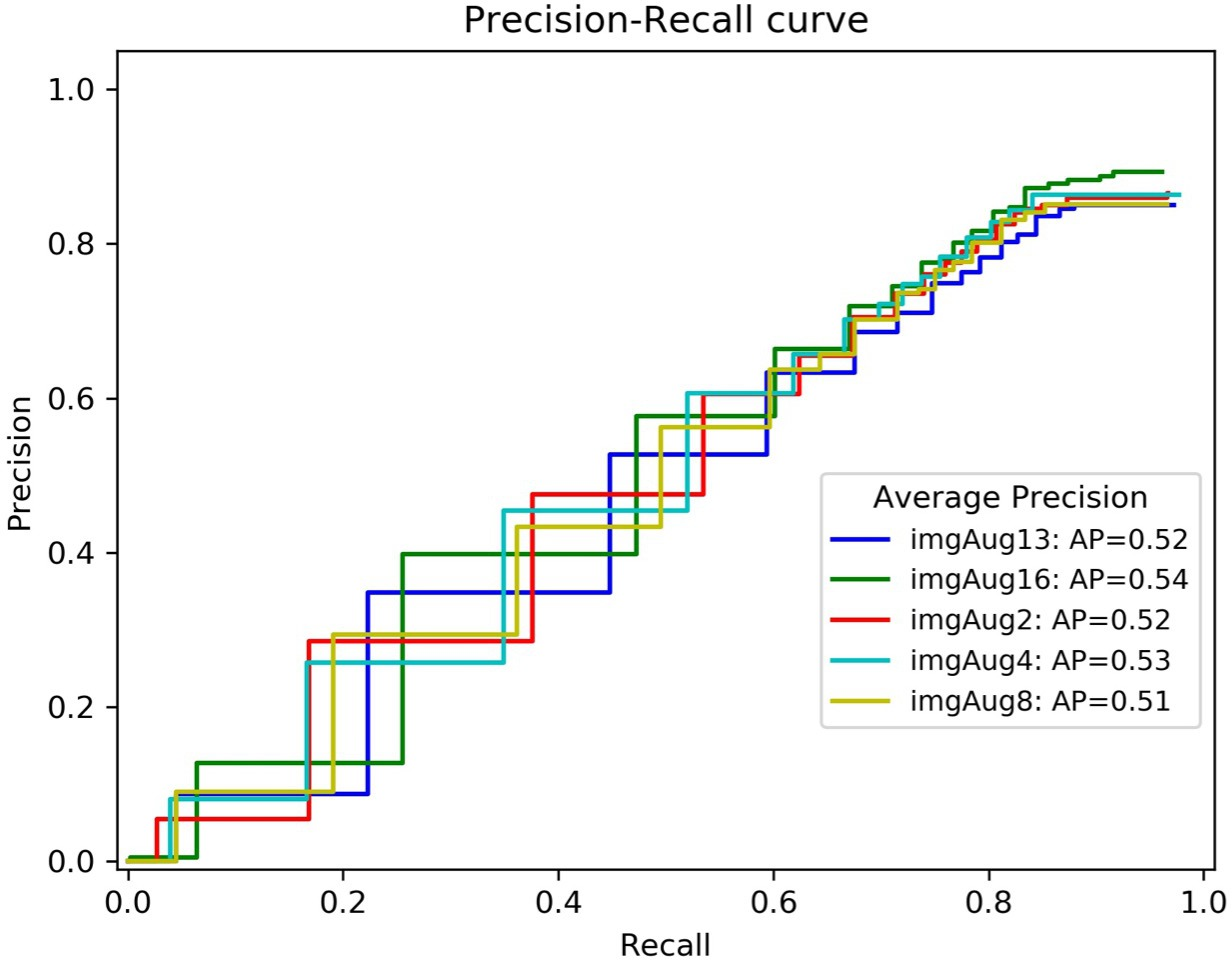
\includegraphics[width=10cm]{figures/top5_curves_trim.jpg}
	\caption{Precision-recall curves of the top five average precision (AP).}
	\label{fig_ap_top5}
\end{figure}

The relation between Precision and recall at various IOU thresholds is almost linear as the precision-recall curves shown in Fig. \ref{fig_ap_top5} as well as Figure S4 and S5 in the Supplementary Materials. The reason is that TP increase and FP (or FN) decrease simultaneously as IOU thresholds decrease. There are distinct steps in precision-recall curves between recall from 0.2 to 0.6. This is because there are only a few mapped polygons with IOU between 0.1 to 0.7 (e.g., Fig. \ref{fig_iou_hist_exp16}).

\begin{figure}
	\centering
	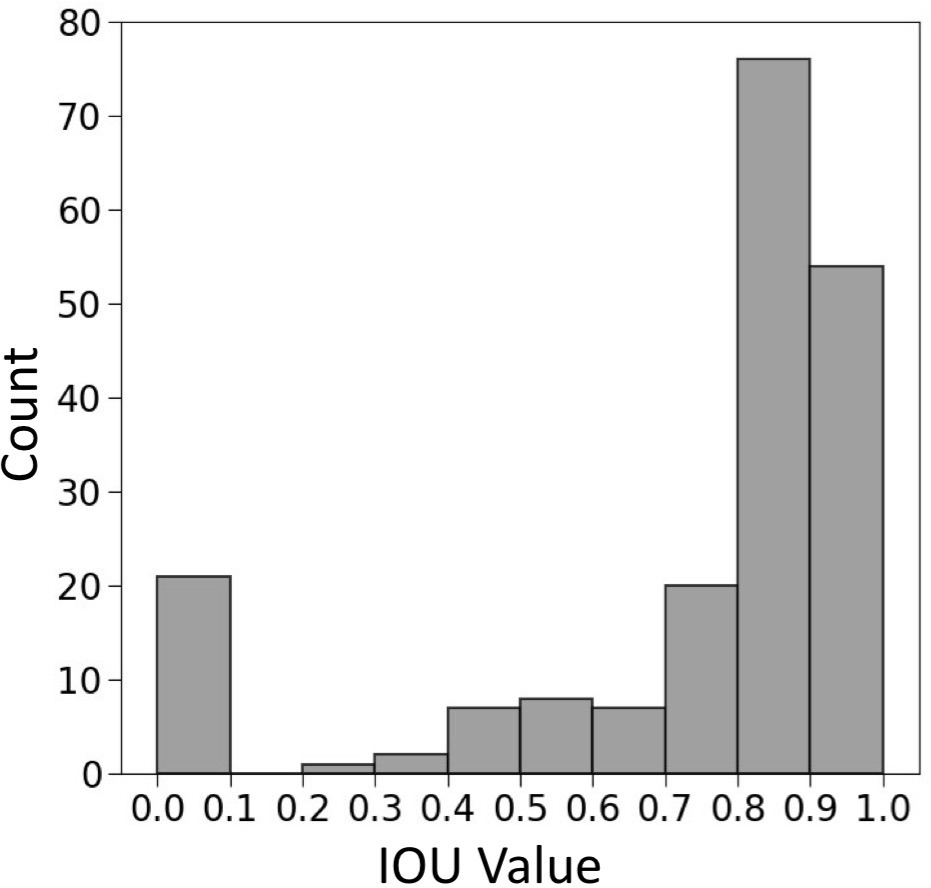
\includegraphics[width=8cm]{figures/IoU_imgAug16_label_trim.jpg}
	\caption{IOU Histogram of mapped polygons in experiment \#16.}
	\label{fig_iou_hist_exp16}
\end{figure}

\subsection{Using different bands of planet images}
\label{subsub_otherbands}

The combination of red, blue, and green bands outperforms other band combination as shown in Table \ref{table_acc_otherbands}. Table \ref{table_acc_otherbands} lists the accuracies of two experiments, which also adopted data augmentation of flipping, blurring, and cropping. The band combination of the experiment \#32 is the blue band of Planet images, normalized difference vegetation index (NDVI), and normalized difference water index (NDWI).  NDVI and NDWI were derived from Planet images. The experiment utilized the first component after principal component analysis (PCA). The AP of \#32 is in the range of Table S1; while \#33 is the lowest. The possible reasons are discussed in section \ref{subsec_advantage_limitation_planet}.  % TODO: move most of the content to method and add why?

\begin{table}[ht]
\footnotesize
\caption{Accuracies of different combination of bands.}
\label{table_acc_otherbands}
%\centering
%% \tablesize{} %% You can specify the fontsize here, e.g. \tablesize{\footnotesize}. If commented out \small will be used.
%\begin{tabular}{cc m{2.2cm}  m{2.2cm}  m{2.2cm} ccc}
\begin{tabular}{c c c c  c ccc c c c c}
\toprule
\textbf{\#}&\textbf{Bands}&\textbf{AP}&\textbf{IOU}&\textbf{TP}&\textbf{FP}&\textbf{FN}&\textbf{Pre}&\textbf{Rec}&\textbf{F1}\\
\midrule

\multirow{3}{*}{32} &  \multirow{3}{*}{B1, NDVI, NDWI} & \multirow{3}{*}{0.514}  &0.8&129&76&73&0.629 &0.639 &0.634   \\
 &  &  &0.4&175&30&25&0.854 &0.875 &0.864  \\
 &  &  &0.0&177&28&6&0.863 &0.967 &0.912   \\

\multirow{3}{*}{33} &  \multirow{3}{*}{1--3 bands after PCA} & \multirow{3}{*}{0.472} &0.8&109&52&93&0.677 &0.540 &0.601  \\
 &  &  &0.4&146&15&53&0.907 &0.734 &0.811  \\
 &  & &0.0&147&14&32&0.913 &0.821 &0.865  \\

\bottomrule
\end{tabular}
\end{table}

\subsection{Accuracies and affecting factors}
\label{subsec_acc_factors}

Despite some false positives and false negatives, the accuracies achieved in this study are sufficient for further analysis. Automatic mapping results using remote sensing images cannot be perfect when comparing to manual delineation on images or in the field. Even manual delineation on images, it requires validation due to the uncertainties of remote sensing images. By comparing the geometric characteristics as well as statistics of terrain factors derived from automatically mapped RTSs and manual delineation (i.e., ground truth), we can conclude they have very high similarity. Therefore, we also use the automatic mapping results for further analysis or updating existing maps, especially in the region where the manually delineated results are unavailable or outdated. 

Polygon-based validation is more practical and understandable than pixel-based validation. We achieve a very high overall accuracy index (i.e., 0.999) because most of the study area are non-RTS, and was corrected labeled as non-RTS pixels. The pixel-based are suitable for comparison with other methods which conduct classification pixel by pixel. However, our targets are the extents of RTSs. Therefore, polygon-based validation is more suitable and meaningful for this study.

The accuracies can be higher if we adjust the criteria of removing mapped polygons or IOU thresholds as we show in Table \ref{table_acc_imgaug}. Different tasks could have different mapping purposes. For example, if the mapping goal is to find the locations of RTSs, a lower threshold of IOU is a good choice. If we lower the threshold of removing small mapped polygons, we may achieve results with no false negatives. For a region without ground truths, we cannot apply the IOU threshold. A practical approach for achieving satisfying results is to lower the criteria of removing false positives, then manually checking mapped polygons on images. 

The delineated accuracies of individual RTSs can be represented by IOU values and affected by many factors. The delineated accuracies are critical for analyzing the temporal change in RTS extents as well as the total mapping accuracies. In this study, we analyzed the relations between IOU values and geometric characteristics of RTSs as well as the count of adjacent RTSs. Figure S8 and S9 in the supplementary materials shows that a small mapped polygon (whose area and perimeter are smaller than most of the polygons) tends to have lower IOU values, but there are also many mapped polygons with high IOU values are small. If the mapped polygons have a larger size, they tend to have higher IOU values. The IOU values don’t correlate with the circularities of RTSs as shown in Figure S10 in the supplementary materials. 

As shown in Figure S11 in the supplementary materials, the count of adjacent RTSs can affect the IOU values. The adjacent RTSs are those RTSs have intersections with the buffer area of a center RTS. Figure S11 only shows the mapped polygons which only cover one RTS. The false positives are those with zero or two adjacent RTSs, and the zeros are the majorities. Many high IOU values also correspond to the zero adjacent RTSs. The reason could be that these RTSs share similar features which are enhanced during training. The setting of buffer areas and overlap pixels in the step of preparation of training images results in the duplication of RTS pixels. If an RTS have more adjacent RTSs, it will have more duplication in the training data. Therefore, the algorithm learns more features of the RTS and be more sensitive to it and similar ones. 

The uncertainty of training polygons some of which are derived from ground truths can also affect the mapping accuracies. The uncertainties include (1) RTSs may be at different stages of development, but we did not distinguish them when collecting and validating the ground truths. (2) many of the RTSs are validated in 2014, but the acquisition date of the images is in 2018. (3) around 10\% of ground truths are used without validation in the field because they are challenging to reach. 

\section{The spatial distribution and terrain factors}
\label{sec_spatial_terrain}

\subsection{The mapped RTSs }
\label{subsub_mapped_rts}

The results with the highest AP are from \#16 in Table \ref{table_acc_imgaug} and contain 196 RTSs, i.e., mapped polygons (Fig. \ref{fig_mapped_rts} and \ref{fig_zoomin_mapped_rts}). With IOU threshold as 0.5, 165 of them are true positives, 31 are false positives, and 37 of the ground truths are missing, i.e., false negatives. The corresponding precision, recall, and F1 score are 0.842, 0.817, and 0.829, respectively. For the pixel-based validation, the Kappa index is 0.917 and overall accuracy index is 0.999. As shown in Fig. \ref{fig_zoomin_mapped_rts}, the automatic-based boundaries match manual-based ones very well, which is consistent as the IOU histogram shown in Fig. \ref{fig_iou_hist_exp16}. The false positives are at the locations where the land covers are quite similar to RTSs. Since some of the RTSs are close to each other (their closest part is less than 15 m, i.e., five pixels), they were merged to one RTS by the mapping method, which leads to that the sum of TP and FN is not equal to the number of ground truths in some experiments (in Table S1). Once a mapped polygon covers two or more RTSs, it can be categorized as either a true positive or false positive (e.g., two examples marked by rectangles in Fig. \ref{fig_zoomin_mapped_rts}a) depend on its IOU value. In experiment \#16, there are 17 mapped polygons, each covers more than two RTSs, cover 37 RTSs in total. Most of the RTSs are in the western part, especially northwestern, of the study area. The possible reason is that the spatial distribution of RTS is limited by permafrost distribution as described in \citealp{yin2017effects}. %TODO: add permafrost exent?

\begin{figure}
	\centering
	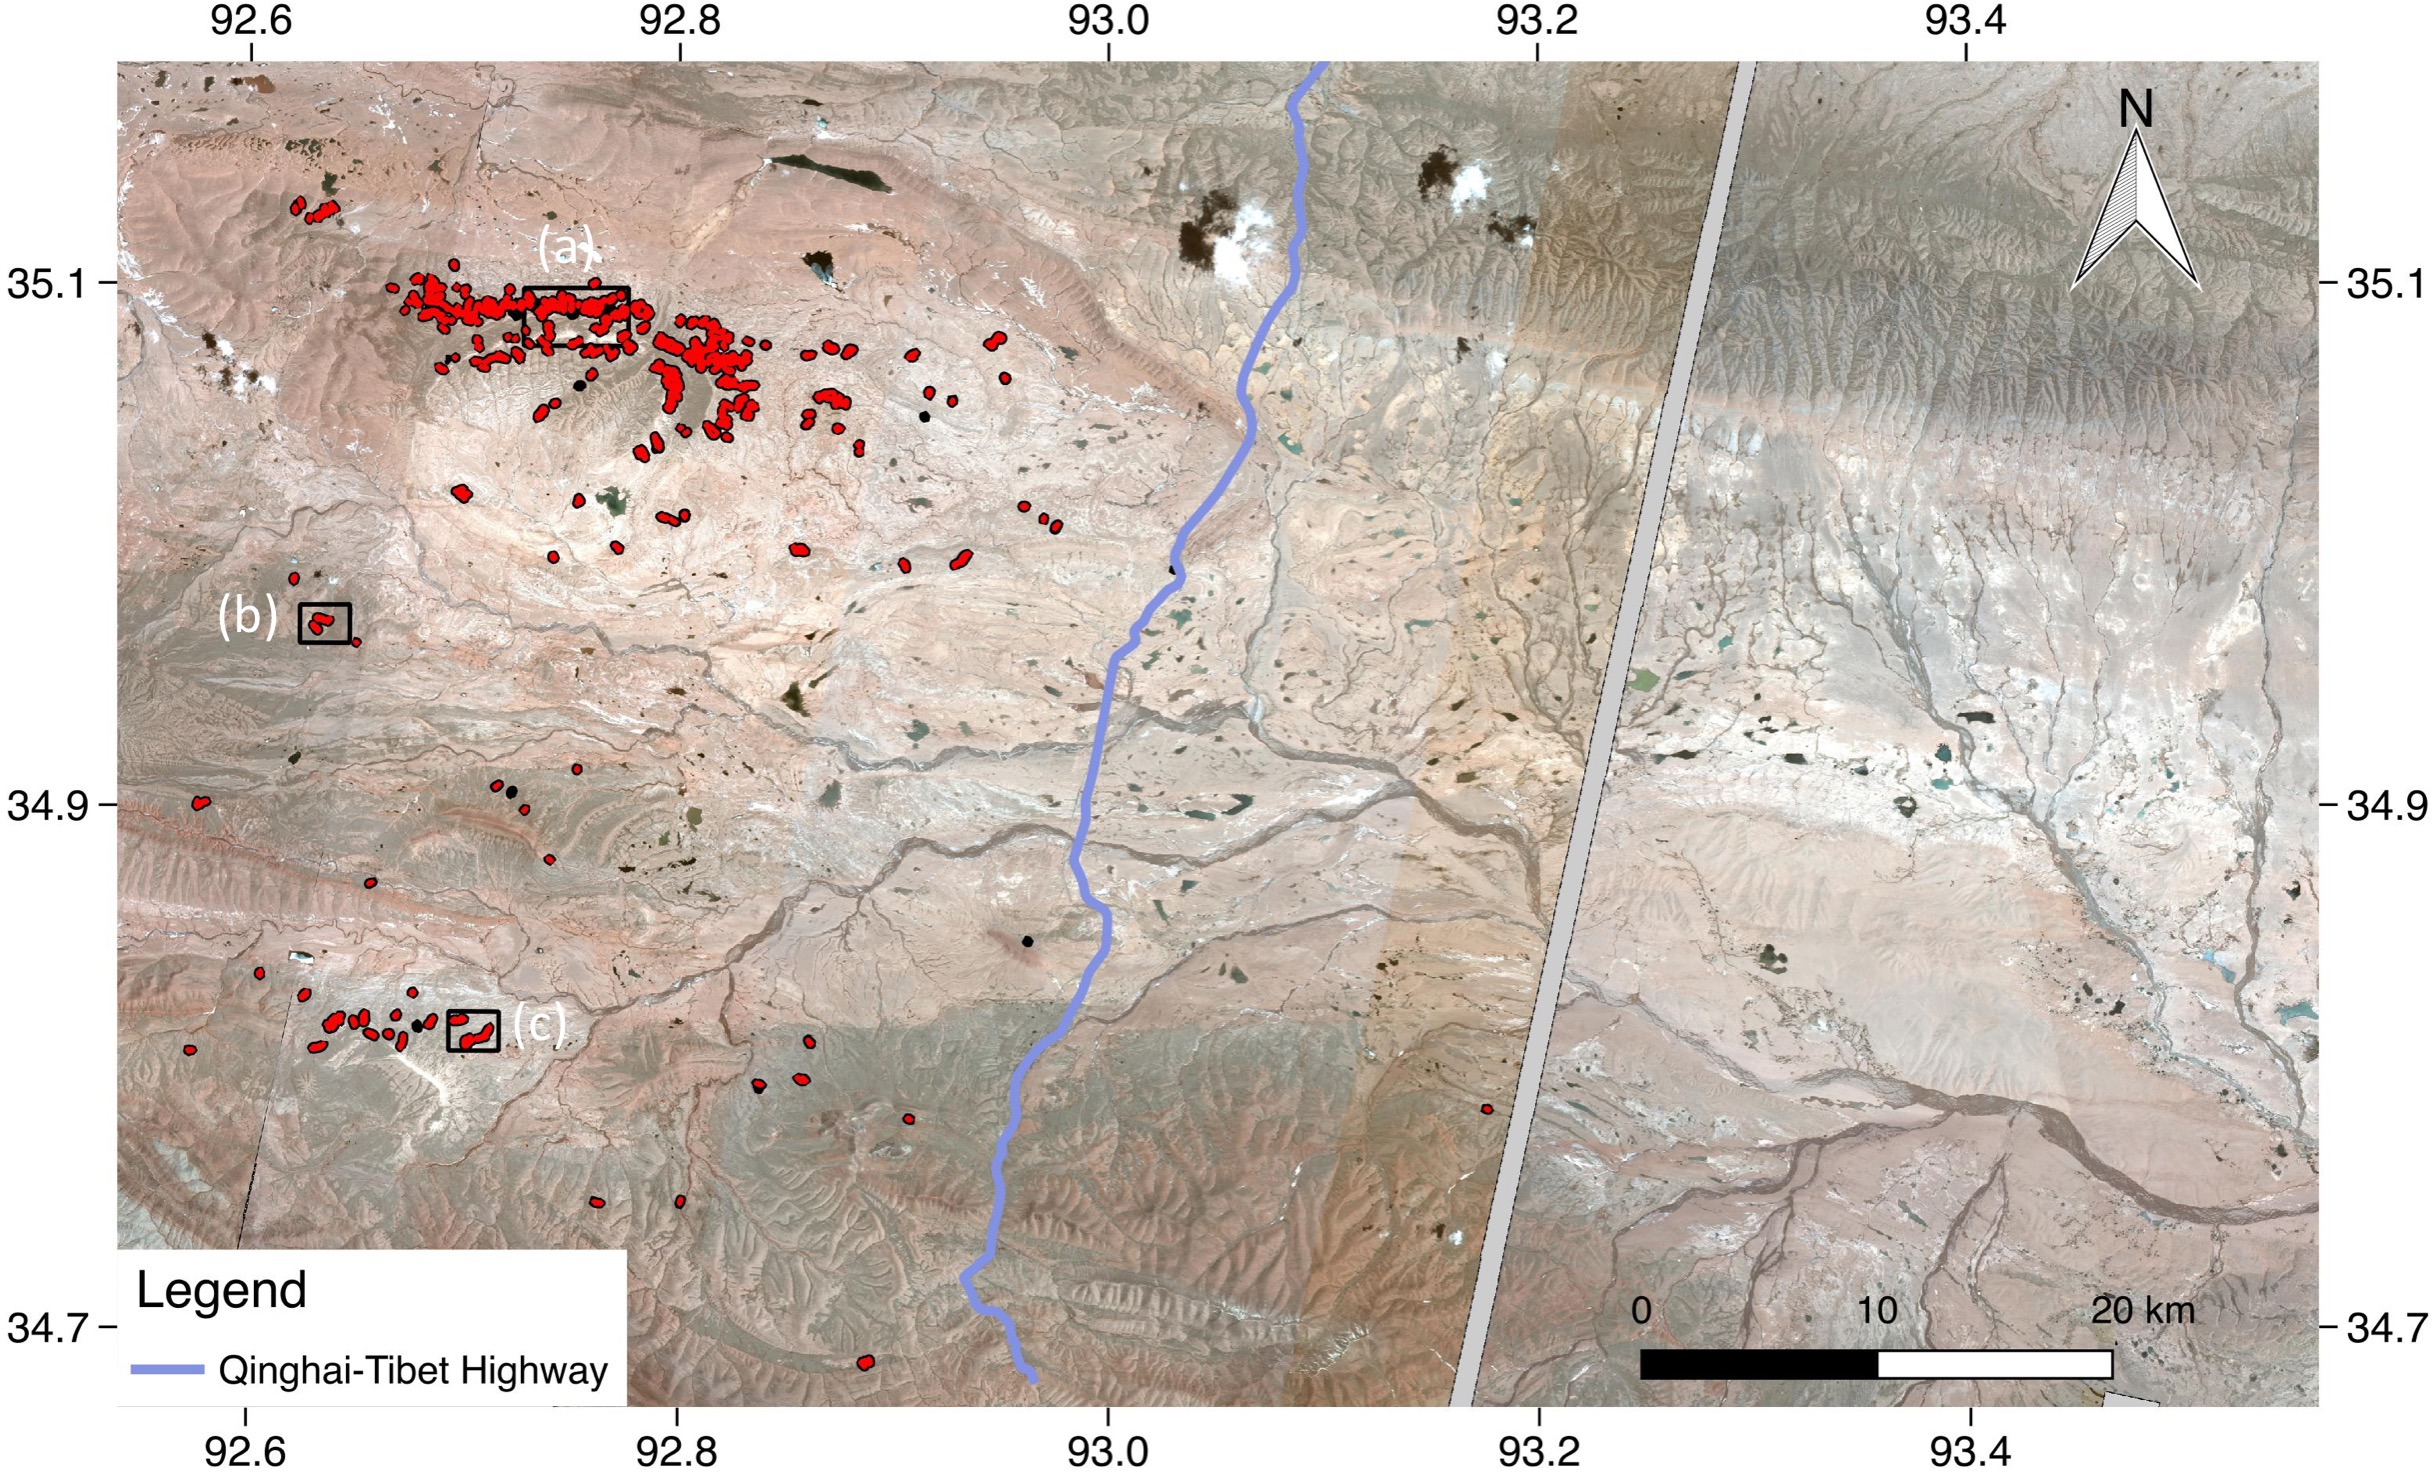
\includegraphics[width=14cm]{figures/whole_area_mapped_trim.jpg}
	\caption{Automatically mapped retrogressive thaw slumps (red or yellow polygons) versus manual delineation (black polygons) on Planet images. The red and yellow polygons are true positives and false positives, respectively.  (a)--(c) are extents of the figures in Fig. \ref{fig_zoomin_mapped_rts}. The gap on the image is due to the lack of Planet scenes}
	\label{fig_mapped_rts}
\end{figure}

\begin{figure}
	\centering
	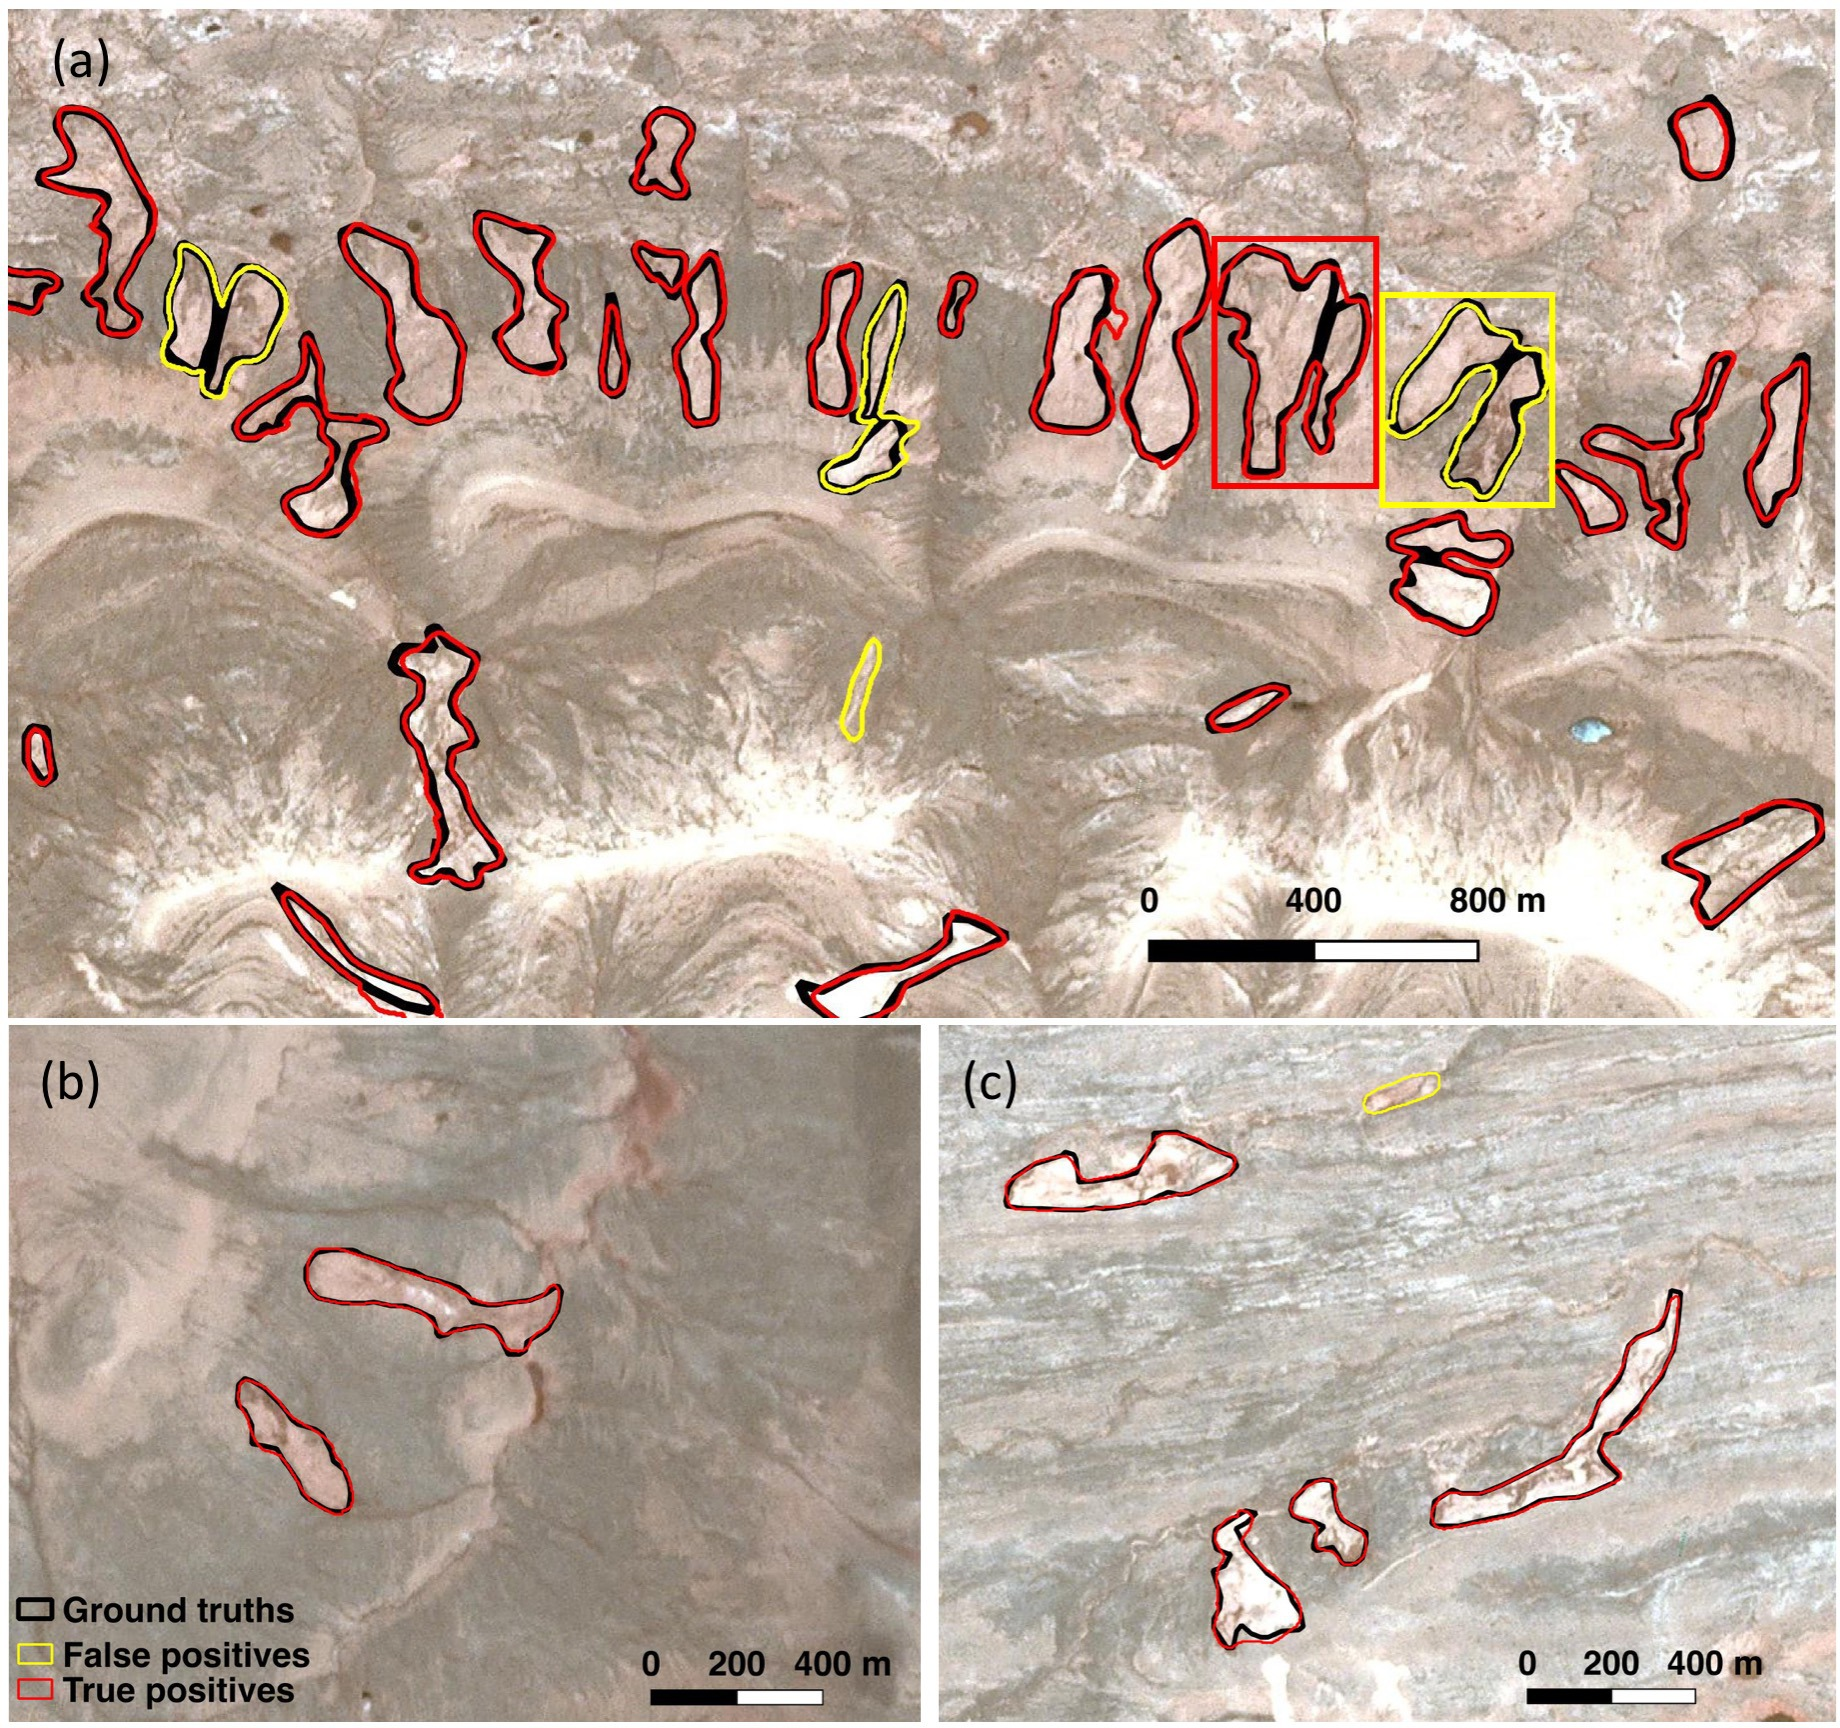
\includegraphics[width=12cm]{figures/zoom_in_mapped_polygons_trim.jpg}
	\caption{Amplifications fo mapping results. (a)--(c) are amplifications of three regions marked by black rectangles in Fig. \ref{fig_mapped_rts}. The two rectangles marked are discussed in section \ref{subsub_mapped_rts} and \ref{subsec_advantage_limitation_method}.}
	\label{fig_zoomin_mapped_rts}
\end{figure}

\subsection{RTS geometric characteristics and terrain factors}
\label{subsub_chara_terrain}

\begin{figure}
	\centering
	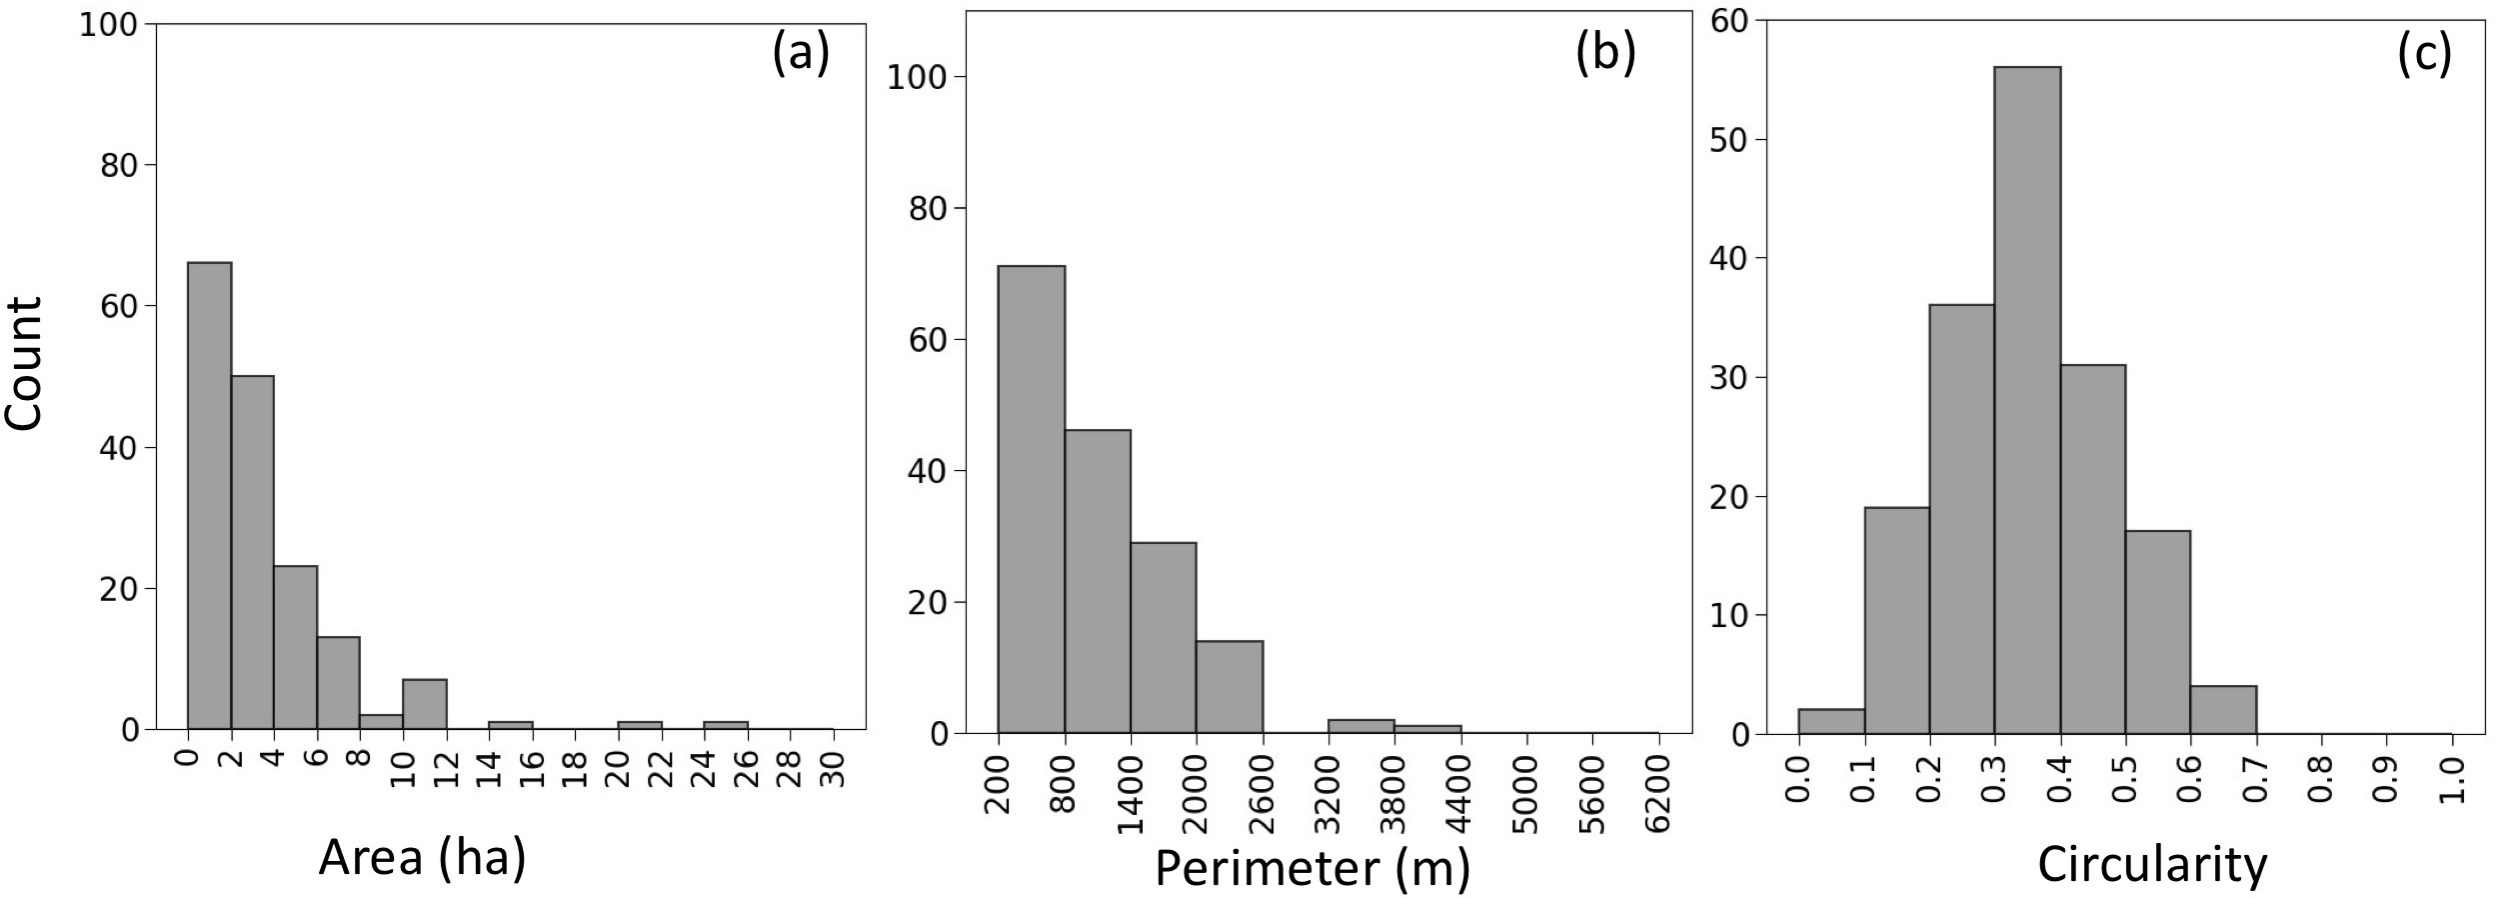
\includegraphics[width=14cm]{figures/geometric_var_mapped_trim.jpg}
	\caption{Geometric statistics of the RTSs based on automatic mapping results (\#16 in Table \ref{table_acc_imgaug}). }
	\label{fig_geometric_statistics}
\end{figure}


Fig. \ref{fig_geometric_statistics} shows the geometric characteristics of mapped RTSs.  The areas of mapped RTSs range from 0.3 to 34.6 ha, with an average of 3.7 ha, and 95\% of them are smaller than eight ha as shown in Fig. \ref{fig_geometric_statistics}a. There is only one mapped RTS whose area is 34.6 ha is not shown in Fig. \ref{fig_geometric_statistics}a because it exceeds the histogram range. Their perimeters range from 288 to 8226 meters, with an average of 1191 meters, and 90\% of them are smaller than 2000 meters as Fig. \ref{fig_geometric_statistics}b. Two of the mapped RTSs, whose perimeters are 6924 meters and 8226 meters, are not shown in Fig. \ref{fig_geometric_statistics}b. Fig. \ref{fig_geometric_statistics}c shows a normal distribution of the circularities with minimum, maximum, and average of 0.06, 0.65, and 0.35, respectively. 

The geometric characteristics of mapped RTSs are quite similar to the ones of ground truths. Figure S6 in the Supplementary Materials shows that the areas, perimeters, circularities of ground truths range from 0.25 to 28.3 ha, 235 to 5898 meters, and 0.1 to 0.9, respectively. Their averages are 3.1 ha, 893 meters, and 0.49, respectively. The averages of areas and perimeters of mapped RTSs are higher than ground truths, but the circularities are lower. The reasons are (1) many small and nearly circle RTSs are missing in the mapped results and (2) some of RTSs are close to each other and merged to one polygon such as the one marked by the red rectangle in Fig. \ref{fig_zoomin_mapped_rts}a.  

\begin{figure}
	\centering
	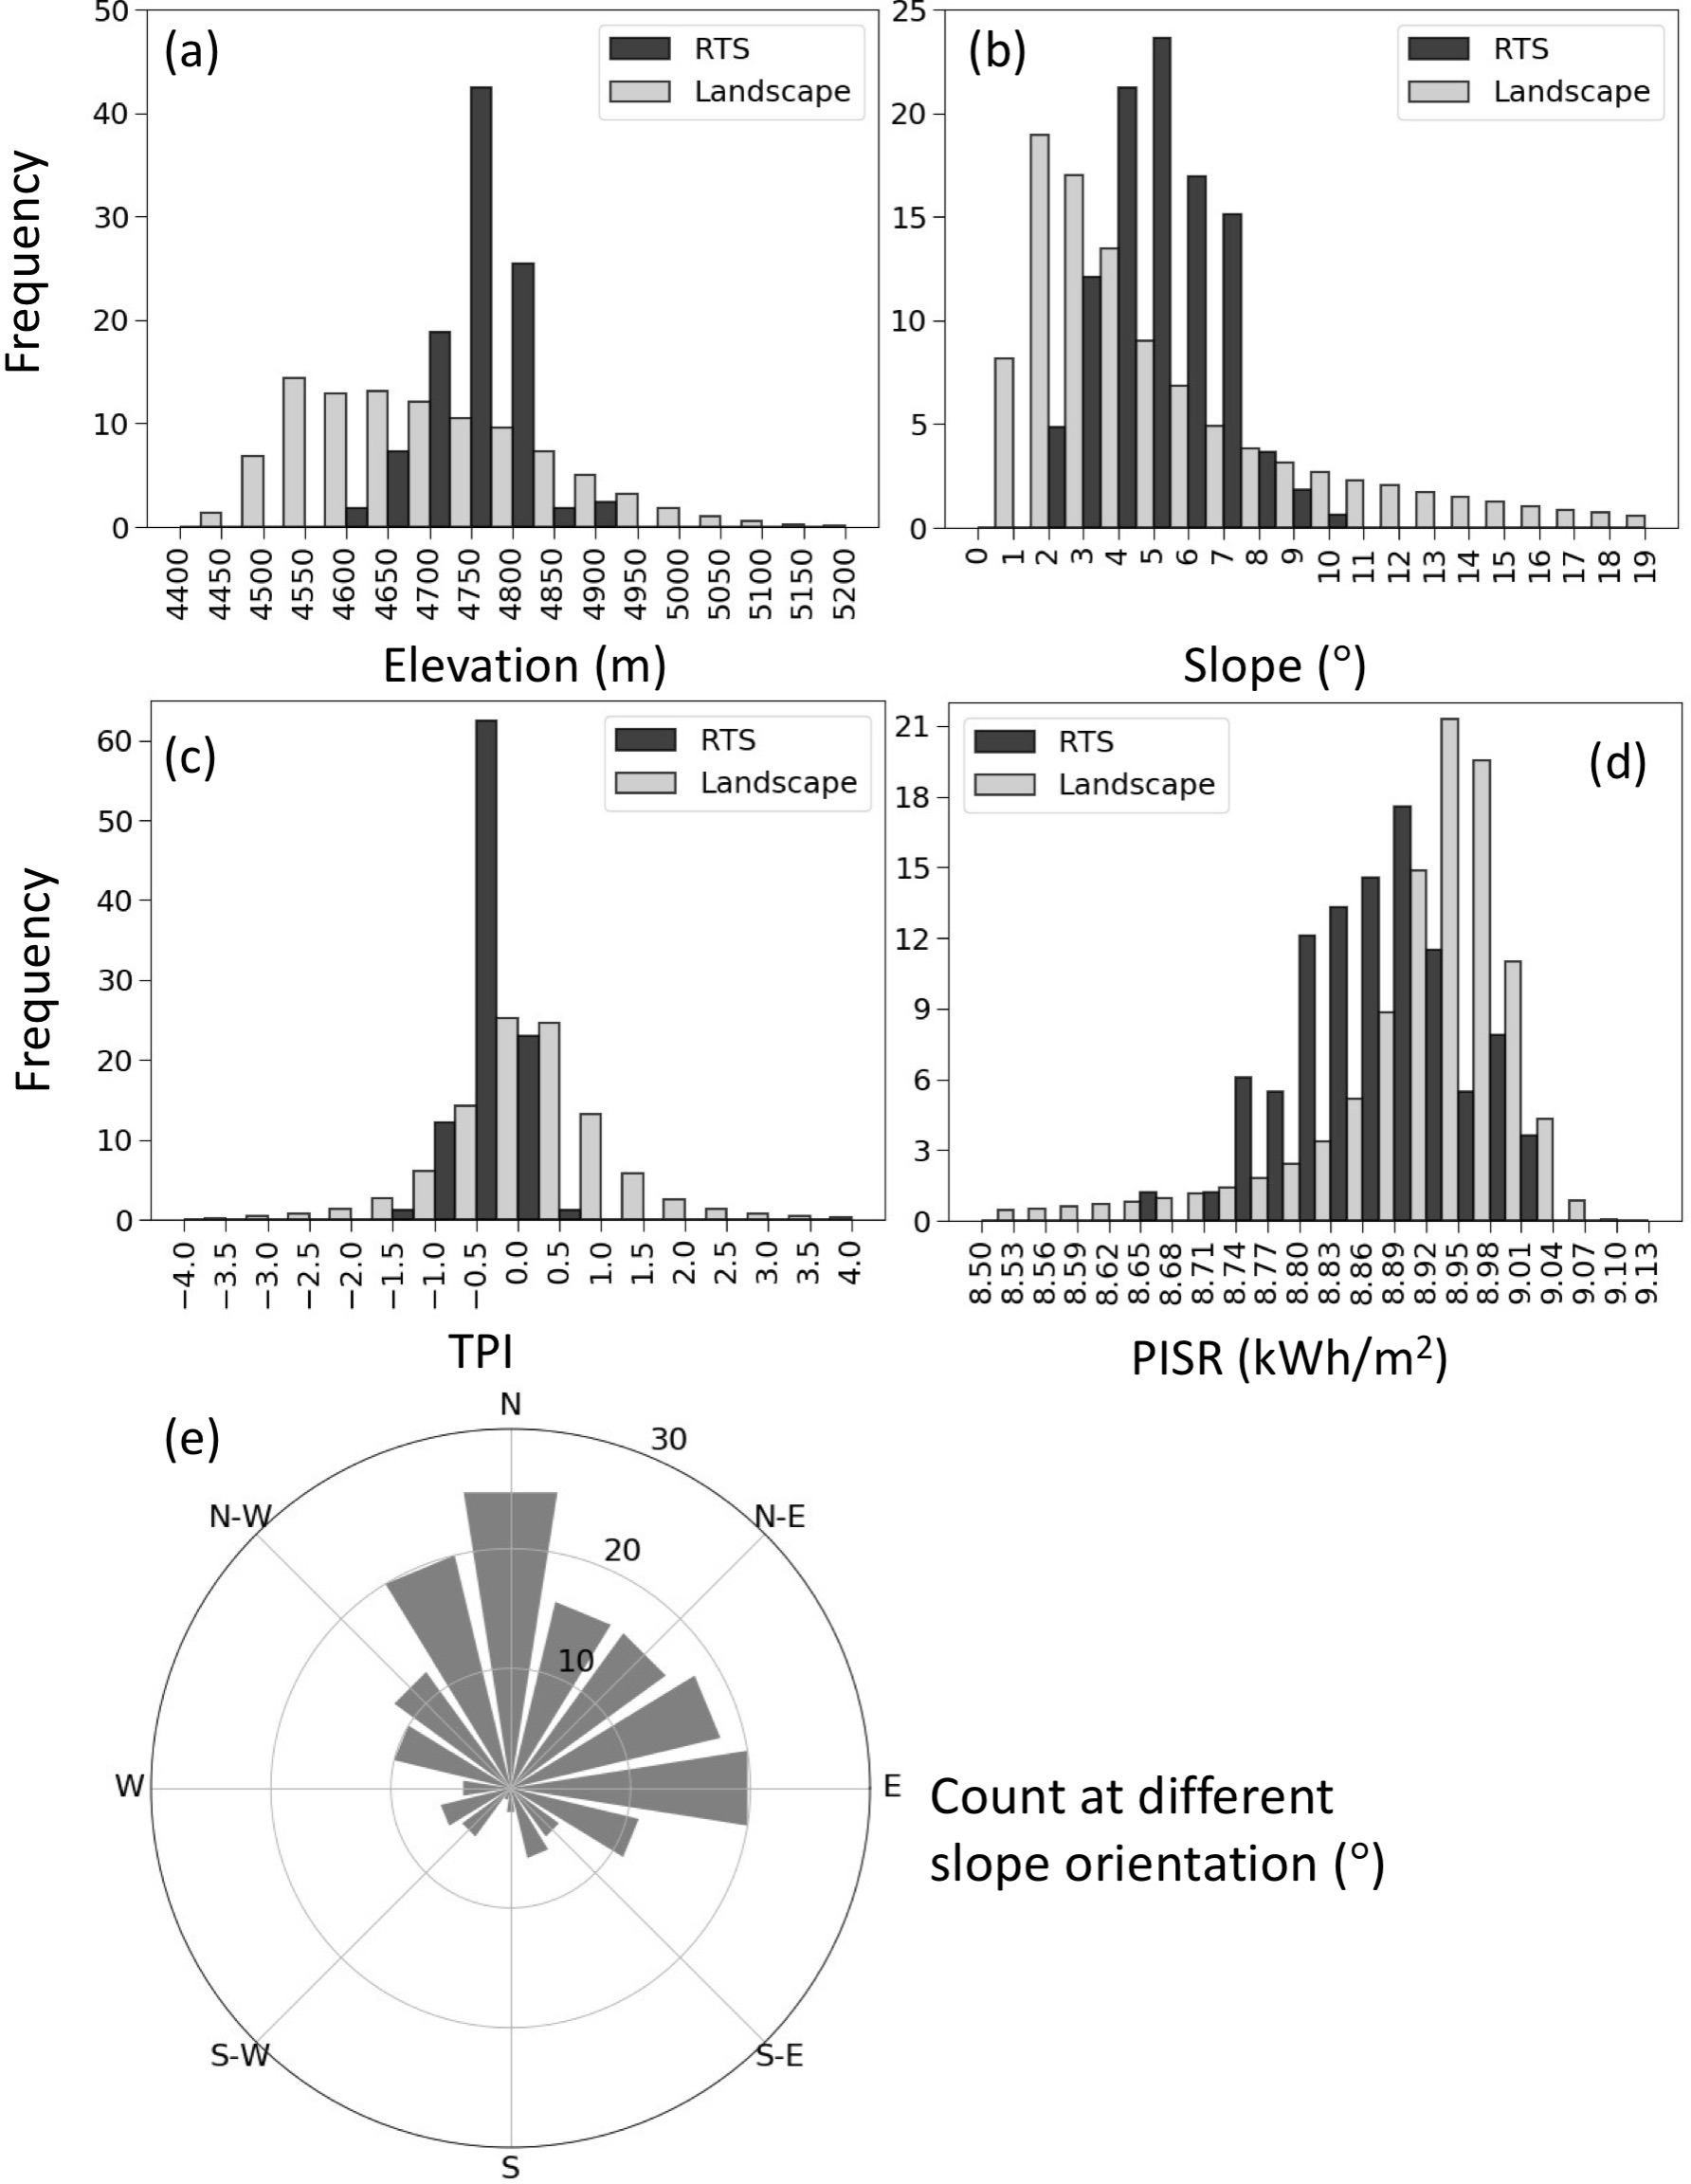
\includegraphics[width=13cm]{figures/terrain_var_fig_mapped_trim.jpg}
	\caption{Statistics of RTS terrain factors based on automatic mapping results  (\#16 in Table \ref{table_acc_imgaug}). }
	\label{fig_terrain_factors}
\end{figure}

Fig. \ref{fig_terrain_factors} shows the occurrences of mapped RTSs regarding different terrain factors. Their elevation and slope range from 4639 meters to 4938 meters and 2.4 degrees to 10.2 degrees, with an average of 4776 meters and 5.6 degrees, respectively. The frequencies in Fig. \ref{fig_terrain_factors}a and b show that RTSs preferentially occur in the elevation from 4700 to 4850 meters and the slope from four to eight degrees, which implies RTSs prefer the gentle slope. The TPI of mapped RTSs range from -1.3 to 0.6 with an average of -0.17 as shown in Fig. \ref{fig_terrain_factors}c, which indicates that most of RTSs in the location slightly lower than their surrounding although they are on the slopes. Their daily PISR in summer varies between 8.65 to 9.04 $kWh/m^2$, with a mean of 8.88 $kWh/m^2$. The frequency in Fig. \ref{fig_terrain_factors}d shows that RTSs preferentially occur at the locations where PISR ranges from 8.74 to 8.92 $kWh/m^2$, which less than majority landscapes.  Their preferential orientations are north and northeast as shown in Fig. \ref{fig_terrain_factors}e, which tend to have less received incoming solar radiation than the south on the Tibetan Plateau. 

Comparison between Fig. \ref{fig_terrain_factors} and Figure S7 in the Supplementary Materials shows that there is no significant difference in occurrences between mapped RTSs and ground truths. The averages of elevation, slope, TPI, and PISR based on the ground truth are 4775 meters, 5.7 meters, --0.15, and 8.88 $kWh/m^2$. The distributions of slope orientations are similar except the total number is reduced because some of the RTSs are missing in the mapped results. 

\subsection{Relation between the RTS spatial distribution and terrain factors}
\label{subsec_spatial_dis_terrain}

We investigated the relation between RTS spatial distribution and terrain factors, including elevation, slope angle as well as orientation, TPI, and PISR. Many factors, including vegetation, soil texture, and ice context can affect the spatial distribution of RTSs as well as permafrost but beyond this study. 

The elevation is the main factor affecting the spatial distribution of RTSs. As shown in Fig. \ref{fig_mapped_rts}, almost all the RTSs are in the west of the Qinghai-Tibet Highway, while the elevation in the west of the Highway is higher than the east as shown in Figure S12 in the supplementary materials. Permafrost on the Tibetan Plateau is known as Plateau Permafrost whose formation is mainly controlled by the elevation. Once the permafrost degradation, it can result in thermokarst landforms including RTSs. Therefore, elevation affects the spatial distribution of permafrost, then limit the spatial distribution of RTSs. However, elevation is not the only factor controlling the distribution of permafrost, other factors such as land cover type also can affect the distribution as the discussion in \citealp{yin2017effects}.

RTSs preferentially occurs on gentle slopes, which have been well discussed in many studies (e.g., \citealp{leibman1995cryogenic, niu2014thaw, lacelle_distribution_2015}). A slope is essential for water and melted materials from permafrost flow downward and keep the permafrost exposed to the air. In permafrost areas, a gentle slope allows water to accumulate under the active layer, then trigger the detachment of the active layer by reducing the friction between uppermost permafrost and the active layer, then exposed the ice-rich permafrost \citep{mcroberts1974stability, mcroberts1974the}. 

The statistics of TIP shows RTSs are common in the location relative lower than their surroundings. The relatively lower position allows water from melting of ground ice or precipitation easy to accumulate, then increase the potential of triggering the detachment of active layers. Lower positions are easy to accumulate snow from precipitation and wind blow in winter. Snow cover can prevent the cooling of permafrost in the winter, which increases the potential of permafrost thawing in the next thawing season. 

Slope orientation and PISR inconsistently show that RTSs are preferentially in the location where received less solar radiation. Less solar radiation can lead to shallower active layers, which increase the likelihood of ground ice being closer to the surface and hence more accessible to thawing. The northern slope may have greater snow accumulation and persistence, which can increase the soil moisture in the thawing season. The reason for more east-facing than west-facing could be that convective clouds commonly between 1200--1800, so higher insolation in the morning than in the afternoon \citep{niu2014thaw}.


\section{Discussion}
\label{sec_discussion}

\subsection{Advantages and limitations of using Planet images}
\label{subsec_advantage_limitation_planet}

Global coverage and high temporal resolution are the advantages of using Planet images. RTSs is the most dramatic dynamic landforms in the permafrost, which requires images with high temporal resolution to monitor their temporal changes. The images from the same sensors would make the pre-processing and analysis of images easier and fewer uncertainties. With the advantage of high temporal resolution, we can collect images without cloud cover for a region in a short period such as one month. Planet also provides the monthly mosaic of cloud-free images. The global coverage of Planet images makes it easy to extend our method to other regions for mapping RTSs without re-training. 

The spatial resolution of Planet images is the main limitation, which results in the missing of many small (less than 0.3 ha) RTSs in the results. Although the Planet images downloaded from the vendor website have a spatial resolution of 3.0 meters, the actual resolution can be lower depends on the parameters of CubeSat such as looking angles. RTSs contains many portions including headwall, slump floor, and slump lobe. The different portions of RTSs may be unable to distinguish even their areas are greater than 0.3 ha. Moreover, if the temporal changes of the RTS are smaller than one pixel of Planet images, then the changes cannot be identified. Although Planet images have four bands, most of the stabilized thaw slumps, which become drier and covered by new vegetation, are similar to the surrounding and hard to be identified.

\subsection{Advantages and limitations of the automatic mapping methods}
\label{subsec_advantage_limitation_method}

The automatic mapping method can potentially be applied to a large region such as Tibetan Plateau and allows us to investigate RTS in an unprecedented quantity and extent. A large portion of permafrost areas where are challenging to reach remain unmapped because manually mapping on high-resolution images are labor-intensive. The automatic mapping methods can overcome this issue although it contains a few false positives and negatives. Furthermore, with the automatic mapping results in a large area, we can analyze the numerous RTSs simultaneously. 

Transfer learning of the method enables us to apply the same methods to other regions by fine-tuning the model. The method is based on deep learning, which has the intrinsic advantages of transfer learning. With the advantage of transfer learning, we can apply the method to other regions even other landforms by collecting the corresponding data, then fine-tuning the method. 

As a supervised learning method, the training processes is time-intensive and requires adjustment of training parameters. We utilized two mainstream GPUs to train the methods in around 10 hours, which is longer than traditional methods such as support vector machines. There are many hyper-parameters need to set during training. Among them, the most important one is the learning rates, which controls the steps of model adjustment. A higher value of learning rates can lead to an explosion of the loss and crash of the training process. But the restart of training process may make it move forward due to the random initiation of input and out layer. A lower value of learning rates requires a much longer time for training. For a large area, the large volume of high-resolution remote sensing images will propose a challenge.

The performance of the methods highly depends on the quantity and quality of training data. The neural network used in this study has a lot of parameters which requires numerous training data. Moreover, wrong training data will result in the wrong features for the methods. The balance of training data is also important because more training data for a specific class can make the method more sensitive to this class. Although the method can learn features automatically, we don’t know what features it learns because of its black-box nature. 

One unsatisfying of this method is that it cannot distinguish two or more RTSs if there are close to each other as shown in Fig. \ref{fig_zoomin_mapped_rts} with rectangular makers. The reasons could be (1) the deep learning algorithm, that is, DeepLabv3+ is not good at captures the edges of the targets and (2) the merging processing of inference patches gives a higher priority to the RTS pixels than non-RTS pixels.

\subsection{Future work}
\label{subsec_future}

Combining other sources of satellites images such as Landsat and Sentinel-2 with Planet images is the key for improving the mapping results and extending to the large regions. Using high-resolution of remote sensing images will face the challenges of a large dataset. Landsat images are valuable for detecting landscape dynamics and mapping RTSs in large permafrost areas \citep{nitze_detection_2016, nitze_landsat-based_2017, nitze2018remote}, but they cannot accurately delineate the boundaries or only target RTSs with large surface area. With Landsat images, we can identify the locations of RTSs, and then delineate the boundaries of RTSs on Planet images. Since RTSs are usually isolated, therefore, we can reduce the volume of Planet images. Moreover, Landsat images are free for research \citep{zhu2019benefits}, but Planet images are available from commercial satellites. Landsat or Sentinel-2 have more than seven bands, which may help reduce false positives. 

We need to improve the deep learning algorithm to utilize the four bands of Planet images and overcome unsatisfying results. Because the deep learning algorithm only accepts three bands, we conduct the experiments of using different combinations of the four bands, but other combinations did not outperform the one of red, green, and blue bands. The four bands of Planet images have more information than three bands. Therefore, the result of the experiments shows that we did not utilize all the band in a correct approach. We should improve the deep learning algorithm or adopt other state-of-the-art algorithms to fully utilize all bands of Planet images. With the correct use of the four bands, we may improve the results. Some of the mapped polygons cover multiple RTSs, this issue needs to be solved in the future. 

Investigating the temporal changes of RTSs and understanding the controlling factors is necessary in future work. RTSs are among the most dynamic landforms in the permafrost areas, their temporal changes are related to the locate climate changes or human activities. 

\section{Conclusions}
\label{sec_conclusion}

We applied a state-of-the-art deep learning algorithm to Planet CubeSat Images and automatically mapped retrogressive thaw slumps in the Beiluhe regions. We conducted many experiments of the mapping methods. One of them (\#16) with the highest average precision (0.536) contains 196 mapped polygons. Among them, 165 are true positives and 31 are false positives when the IOU threshold is 0.5, and the corresponding precision, recall, and F1 score are 0.842, 0.817, and 0.829, respectively. There are 37 RTSs missing in this result, but only one RTS is truly missing if we lower the criteria of removing small mapped polygons and set the IOU threshold as zero. Even in some experiments, there is no truly missing of RTS (Table S2). The statistics of true positives shows that 95\% of mapped RTSs are smaller than eight ha, and 90\% of their perimeters are smaller than 2000 meters. The comparison between statistics of true positives and manual delineations shows that automatically mapped results show similar statistics to manual ones. Analysis of the terrain factors indicates that (1) RTSs preferentially occur in the locations with relatively high elevation and gentle slopes, (2) the locations where RTSs were triggered are relatively lower than their surroundings, suggested by the statistics of TPI values, and (3) the locations with less received solar radiation, such as north-facing slope have more potential for development of RTSs. This study demonstrates that (1) the method can automatically map RTSs and (2) Planet images are useful for mapping RTSs on the Tibetan Plateau. Although the results contain some false positives and miss a few RTSs, we can conduct analysis based this results and derived a similar conclusion to the one based on manual delineation. 

In the future, we will conduct the analysis of RTS spatial distribution by including more factors such as vegetation and soil texture. We also need to improve the deep learning algorithm to correctly utilize the four bands of Planet images and overcome the multiple overlap issues of mapped polygons, by borrow news ideas from new deep learning algorithms since they develop very quickly. We will extend the method to a large region by combing multiple sources of satellite images and Planet images. The temporal change of RTSs is also one of the main tasks in the future. 

\section{Data and codes}
\label{sec_data_codes}

Data are available on \hl{somewhere}  % TODO: add data link

Codes are available on Github (\url{https://github.com/yghlc/Landuse\_DL}) after publish. 

\section{Acknowledgments}
\label{sec_acknowledgments}

Thanks for Planet’s Education and Research Program, through which we obtained Planet CubeSat Images for this study. We acknowledge the support of NVIDIA Corporation with the donation of a Quadro P5000 GPU used for this research, the Hong Kong Research Grants Council (CUHK14300815), and CUHK Direct Grant for Research (4053282). Lingcao Huang was supported by the CUHK Global Scholarship Programme for Research Excellence when he visited the University of Alberta and conducted this research.



%% The Appendices part is started with the command \appendix;
%% appendix sections are then done as normal sections
%% \appendix

%% \section{}
%% \label{}

\section{References}
\label{sec_reference}

%% If you have bibdatabase file and want bibtex to generate the
%% bibitems, please use
%%
\bibliographystyle{elsarticle-harv} 
\bibliography{03_mapping_RTS_dl_beiluhe.bib}

%% else use the following coding to input the bibitems directly in the
%% TeX file.

%\begin{thebibliography}{00}
%
%%% \bibitem[Author(year)]{label}
%%% Text of bibliographic item
%
%\bibitem[ ()]{}
%\end{thebibliography}


\end{document}

\endinput
%%
%% End of file `elsarticle-template-harv.tex'.
